% =============================================================================
% main.tex — Thesis defense deck (15 min) | HQC on RISC-V via ISA extensions
% Build: latexmk -lualatex main.tex   (handout: see Makefile target `handout`)
% =============================================================================
\documentclass[aspectratio=169,10pt]{beamer}
% =============================================================================
% preamble.tex — HQC-on-RISC-V defense deck (LuaLaTeX + moloch)
% Authored by @Skill — Beamer Presentation Builder.
% Engine: LuaLaTeX (build via latexmk). No TeX engine in sandbox -> static only.
% =============================================================================

\usetheme{moloch}                    % maintained fork of metropolis (pgfplots/TikZ-safe)
% Fraction-style frame numbering (current/total). moloch removed metropolis'
% \metroset/numbering option in favour of beamer's native template, so set it
% directly (the legacy `numbering=fraction` option is deprecated in moloch).
\setbeamertemplate{page number in head/foot}[totalframenumber]

% --- Fonts & language -----------------------------------------------------
% moloch does NOT auto-handle Fira -> set an explicit Greek-capable font.
\usepackage{fontspec}
\usepackage{polyglossia}
\setdefaultlanguage{greek}
\setotherlanguage{english}
\setmainfont{Noto Sans}
\setsansfont{Noto Sans}
\setmonofont{DejaVu Sans Mono}[Scale=MatchLowercase]
\newcommand{\en}[1]{\textenglish{#1}}      % english spans (= \textenglish)

% --- Math -----------------------------------------------------------------
\usepackage{unicode-math}
\setmathfont{Latin Modern Math}             % full Greek + math coverage

% --- Numbers / units ------------------------------------------------------
\usepackage{siunitx}
\sisetup{group-separator={.},group-minimum-digits=4,detect-all}

% --- Tables / lists / code ------------------------------------------------
\usepackage{booktabs}
\usepackage{tabularray}
\usepackage{listings}
\usepackage{pifont}

% --- TikZ / plots ---------------------------------------------------------
\usepackage{tikz}
\usepackage{pgfplots}
\pgfplotsset{compat=1.18}
\usetikzlibrary{positioning,arrows.meta,fit,backgrounds,shapes.geometric,calc}
\usepgfplotslibrary{groupplots}
% Externalization: stable, deterministic figure names (same convention as thesis)
\usetikzlibrary{external}
\tikzexternalize[prefix=build/ext/]

% --- Bibliography ---------------------------------------------------------
\usepackage[backend=biber,style=ieee,sorting=none]{biblatex}
\addbibresource{../bibliography/references.bib}

% --- Semantic, colorblind-safe colors (WCAG AA >= 4.5:1) ------------------
\definecolor{posc}{HTML}{1B7837}\newcommand{\pos}[1]{\textcolor{posc}{#1}}
\definecolor{conc}{HTML}{B2182B}\newcommand{\con}[1]{\textcolor{conc}{#1}}
\definecolor{hlc}{HTML}{2166AC}\newcommand{\HL}[1]{\textcolor{hlc}{\textbf{#1}}}
\definecolor{accent}{HTML}{2166AC}

% =============================================================================
% Macros — class-agnostic subset replicated from preamble/macros.tex
% (NEVER blanket-\input the thesis preamble: scrbook != beamer class coupling)
% Names kept identical to thesis (D-TERM).
% =============================================================================
\usepackage{xspace}
% Mathematical notation
\newcommand{\GF}[1]{\mathrm{GF}(#1)}
\newcommand{\GFpoly}{\GF{2}[x]}
\newcommand{\GFquot}[1]{\GF{2}[x]/(x^{#1}-1)}
\newcommand{\xorop}{\oplus}
% HQC-specific
\newcommand{\HQC}{\textsc{HQC}\xspace}
\newcommand{\KEM}{\textsc{KEM}\xspace}
\newcommand{\KeyGen}{\textsc{KeyGen}\xspace}
\newcommand{\Encaps}{\textsc{Encaps}\xspace}
\newcommand{\Decaps}{\textsc{Decaps}\xspace}
% RISC-V instructions
\newcommand{\insn}[1]{\texttt{#1}\xspace}
\newcommand{\clmul}{\insn{clmul}}
\newcommand{\clmulh}{\insn{clmulh}}
\newcommand{\vclmul}{\insn{vclmul.vv}}
\newcommand{\vclmulh}{\insn{vclmulh.vv}}
\newcommand{\vror}{\insn{vror}}
\newcommand{\rori}{\insn{rori}}
% RISC-V extensions
\newcommand{\ext}[1]{\textsf{\textbf{#1}}}
\newcommand{\Zbc}{\ext{Zbc}\xspace}
\newcommand{\Zbb}{\ext{Zbb}\xspace}
\newcommand{\Zvbc}{\ext{Zvbc}\xspace}
\newcommand{\Zvbb}{\ext{Zvbb}\xspace}
\newcommand{\RVV}{\ext{RVV}\xspace}
% Performance metrics
\newcommand{\instret}{\texttt{instret}\xspace}
\newcommand{\VLEN}{\texttt{VLEN}\xspace}
\newcommand{\VLMAX}{\texttt{VLMAX}\xspace}
\newcommand{\SEW}{\texttt{SEW}\xspace}
\newcommand{\LMUL}{\texttt{LMUL}\xspace}
% Abbreviations
\newcommand{\ie}{i.e.\@,\xspace}
\newcommand{\eg}{e.g.\@,\xspace}
% Emphasis / code
\newcommand{\defterm}[1]{\textbf{\textit{#1}}}
\newcommand{\code}[1]{\texttt{#1}}
\newcommand{\BigO}[1]{\mathcal{O}(#1)}
% Results & measurements
\newcommand{\speedup}[1]{$\times$#1}
\newcommand{\pct}[1]{\SI{#1}{\percent}}
\providecommand{\checkmark}{\ding{51}}

% --- listings style (RISC-V-ish, ASCII only) ------------------------------
\lstdefinestyle{riscv}{
  basicstyle=\ttfamily\scriptsize,
  keywordstyle=\color{accent}\bfseries,
  commentstyle=\color{gray},
  morekeywords={clmul,clmulh,vclmul,vclmulh,vror,vsll,vsrl,vor,vxor,rori,andn,sh3add,bset,slli,add,xor},
  showstringspaces=false,
  columns=fullflexible,
  keepspaces=true,
}
\lstset{style=riscv}

% --- Constant-time content toggle: set \includeCTtrue to restore CT slides ---
\newif\ifincludeCT
\includeCTfalse


\title{Επιτάχυνση του Μετα-Κβαντικού KEM \HQC σε Αρχιτεκτονική RISC-V}
\subtitle{μέσω Επεκτάσεων \en{ISA}}
\author{Φραϊδάκης Ιωάννης \\ {\footnotesize ΑΕΜ 10736}}
\institute{%
  Πολυτεχνική Σχολή · Τμήμα ΗΜΜΥ · Α.Π.Θ.\\[0.6em]
  {\footnotesize Επίβλεψη: Ι. Παπαευσταθίου, Καθηγητής}\\
  {\footnotesize Εξεταστική επιτροπή: Ι. Παπαευσταθίου, Β. Παυλίδης, Α. Χατζόπουλος}%
}
\date{Θεσσαλονίκη, Ιούνιος 2026}

\begin{document}

\maketitle

\begin{frame}{Δομή της παρουσίασης}
  \tableofcontents
\end{frame}

\section{Κίνητρο \& Υπόβαθρο}
% --- 01 Motivation: quantum threat -------------------------------------------
\begin{frame}{Η κβαντική απειλή}
  \begin{columns}[T,onlytextwidth]
    \begin{column}{0.56\textwidth}
      \begin{itemize}
        \item Ο αλγόριθμος του \en{Shor} σπάει \en{RSA} / \en{ECC} σε πολυωνυμικό χρόνο~\cite{Shor1997}
        \item \HL{“\en{Harvest now, decrypt later}”}: τα δεδομένα κλέβονται σήμερα, αποκρυπτογραφούνται αύριο
        \item Εντολή \en{NSA CNSA 2.0}: μετάβαση σε \en{PQC} έως το \HL{2035}~\cite{NSA-CNSA2}
      \end{itemize}
      \vspace{0.6em}
      \pause
      \begin{block}{Γιατί \HQC;}
        Τον Μάρτιο 2025 το \en{NIST} επέλεξε το \HQC ως πρότυπο \en{KEM}, εναλλακτικό στο \en{ML-KEM}, βασισμένο σε κωδικοθεωρία~\cite{NIST-HQC-selection2025}.
      \end{block}
    \end{column}
    \begin{column}{0.44\textwidth}
      \begin{exampleblock}{Διαφοροποίηση κινδύνου}
        Το \HQC στηρίζεται σε \emph{διαφορετική} υπόθεση σκληρότητας (αποκωδικοποίηση συγκλινούσας) απ' ό,τι τα πλεγματικά, αντιστάθμιση σε μια μελλοντική κρυπτανάλυση.
      \end{exampleblock}
    \end{column}
  \end{columns}
\end{frame}

% --- 02 HQC KEM in one slide -------------------------------------------------
\begin{frame}{Το \HQC σε μια διαφάνεια}
  \begin{columns}[T,onlytextwidth]
    \begin{column}{0.5\textwidth}
      \textbf{Βασικά στοιχεία}
      \begin{itemize}
        \item \en{Code-based} \KEM στον δακτύλιο $\GFquot{N}$
        \item Αριθμητική στο \GFpoly: πολλαπλασιασμός αραιών × πυκνών πολυωνύμων
        \item Διόρθωση σφαλμάτων: συνελισσόμενοι \en{Reed--Muller} + \en{Reed--Solomon}
        \item \en{IND-CCA2} μέσω μετασχηματισμού \en{Fujisaki--Okamoto}~\cite{FujisakiOkamoto1999}
      \end{itemize}
    \end{column}
    \begin{column}{0.5\textwidth}
      \textbf{Ροή \KEM}
      \begin{enumerate}
        \item \KeyGen: $(\mathit{pk},\mathit{sk})$
        \item \Encaps: $\mathit{pk}\rightarrow(\mathit{ct},K)$
        \item \Decaps: $\mathit{ct},\mathit{sk}\rightarrow K$
      \end{enumerate}
      \vspace{0.4em}
      \begin{alertblock}{Κρίσιμο για την ασφάλεια}
        Όλες οι πράξεις πρέπει να είναι \HL{σταθερού χρόνου} (\en{constant-time}) — καμία εξάρτηση από μυστικά δεδομένα.
      \end{alertblock}
    \end{column}
  \end{columns}
  \vspace{0.3em}
  {\footnotesize Παράμετροι: \HQC-128/192/256 ($N=\num{17669}/\num{35851}/\num{57637}$). Βλ. παράρτημα.}
\end{frame}

% --- 03 RISC-V platform & relevant extensions --------------------------------
\begin{frame}{RISC-V: ανοιχτό \en{ISA} με κρυπτογραφικές επεκτάσεις}
  \begin{itemize}
    \item Αρθρωτή, ανοιχτή \en{ISA}, ιδανικό πεδίο για εξειδικευμένη επιτάχυνση
  \end{itemize}
  \vspace{0.4em}
  \begin{columns}[T,onlytextwidth]
    \begin{column}{0.5\textwidth}
      \begin{block}{Βαθμωτές (σειριακές)}
        \begin{itemize}
          \item \Zbc: \clmul / \clmulh, πολ/σμός χωρίς κρατούμενο στο \GFpoly
          \item \Zbb: περιστροφές/λογικές για \en{Keccak}
        \end{itemize}
      \end{block}
    \end{column}
    \begin{column}{0.5\textwidth}
      \begin{block}{Διανυσματικές (\en{RVV})}
        \begin{itemize}
          \item \Zvbc: \vclmul / \vclmulh, διανυσματικός πολ/σμός
          \item \Zvbb: \vror, διανυσματικές λογικές για \en{Keccak}
        \end{itemize}
      \end{block}
    \end{column}
  \end{columns}
  \vspace{0.4em}
  \pause
  \begin{exampleblock}{Τρεις βαθμίδες ανάπτυξης (\en{deployment tiers})}
    \HL{Βαθμίδα 1}: σειριακή (\Zbc/\Zbb) ·\quad
    \HL{Βαθμίδα 2}: βασική \RVV ·\quad
    \HL{Βαθμίδα 3}: \en{vector-crypto} (\Zvbc/\Zvbb)
  \end{exampleblock}
  \vspace{-0.2em}
  {\footnotesize Προφίλ \en{RVA23}~\cite{RVA23-profile}: οι κρυπτογραφικές επεκτάσεις γίνονται υποχρεωτικές.}
\end{frame}


\section{Πρόβλημα \& Προσέγγιση}
% --- 04 Problem (fullbleed, L): pie-dominant, standfirst + minimal κείμενο ----
\begin{frame}{Ο πολυωνυμικός πολ/σμός κυριαρχεί: $\sim\!\pct{97}$ του κόστους}
  \vspace{0.5em}
  \HL{Σχεδόν όλο το κόστος του \HQC-128 συγκεντρώνεται σε έναν πυρήνα.}
  \vfill
  \begin{center}
    \adjustbox{max width=0.95\linewidth,max height=0.62\textheight,center}{\tikzsetnextfilename{ch2-background-pie-scalar-ref}
\begin{tikzpicture}[
    every node/.style={font=\sffamily},
]

% --- Palette via canonical component tokens (cross-figure consistency) ---
\colorlet{colMul}{figkPolymul}
\colorlet{colKeccak}{figkKeccak}
\colorlet{colDecode}{figkDecode}
\colorlet{colMem}{figkMisc}
\colorlet{colOther}{black!20}
\colorlet{textmain}{black!75}
\colorlet{textsub}{figneutral}

% --- Parameters ---
\def\mainCX{0}
\def\mainCY{0}
\def\outerR{2.8}
\def\innerR{1.7}

\def\insetCX{7.4}
\def\insetCY{0}
\def\insetOuterR{2.0}
\def\insetInnerR{1.1}

% Helper: ring sector
\newcommand{\ringsector}[7]{%
    \fill[#7, draw=white, line width=1.2pt]
        ([shift={(#1,#2)}] #5:#3) arc (#5:#6:#3)
        -- ([shift={(#1,#2)}] #6:#4) arc (#6:#5:#4) -- cycle;
}

% MAIN DONUT (left)
% Multiplication (schoolbook+karatsuba+gf_mul+gf_square+vect_mul+clmul) = 96.61%
% Memory/Utility (memset+memcpy+support_contains_value+vect_*) = 2.07%
% Keccak (KeccakF1600+keccak_inc_*+sha3_*+shake256_*+xof_*+hash_*+prng_*) = 0.76%
% Decode (hadamard+expand_and_sum+gf_reduce+find_peaks+RS/RM+FFT+...) = 0.54%
% Other = 0.01%
\ringsector{\mainCX}{\mainCY}{\innerR}{\outerR}{90}{-257.8}{colMul}
\ringsector{\mainCX}{\mainCY}{\innerR}{\outerR}{-257.8}{-265.2}{colMem}
\ringsector{\mainCX}{\mainCY}{\innerR}{\outerR}{-265.2}{-268.0}{colKeccak}
\ringsector{\mainCX}{\mainCY}{\innerR}{\outerR}{-268.0}{-269.9}{colDecode}
\ringsector{\mainCX}{\mainCY}{\innerR}{\outerR}{-269.9}{-270}{colOther}

\pgfmathsetmacro{\mulMidAngle}{(90 + (-257.8))/2}
\pgfmathsetmacro{\mulLabelR}{(\innerR + \outerR)/2}
\node[font=\sffamily\bfseries\small, text=white] at
    ([shift={(\mainCX,\mainCY)}] \mulMidAngle:\mulLabelR) {96.6\%};

\node[font=\sffamily\bfseries\large, text=textmain] at (\mainCX, \mainCY+0.15)
    {HQC-128};
\node[font=\sffamily\small, text=textsub] at (\mainCX, \mainCY-0.25)
    {Scalar Reference};

% INSET DONUT (right) — Remaining 3.38% expanded (proportional to 360 deg)
% Mem: 2.07/3.38 => 220.5 deg
% Keccak: 0.76/3.38 => 80.9 deg
% Decode: 0.54/3.38 => 57.5 deg
% Other: 0.01/3.38 => remainder
\ringsector{\insetCX}{\insetCY}{\insetInnerR}{\insetOuterR}{90}{-130.5}{colMem}
\ringsector{\insetCX}{\insetCY}{\insetInnerR}{\insetOuterR}{-130.5}{-211.4}{colKeccak}
\ringsector{\insetCX}{\insetCY}{\insetInnerR}{\insetOuterR}{-211.4}{-268.9}{colDecode}
\ringsector{\insetCX}{\insetCY}{\insetInnerR}{\insetOuterR}{-268.9}{-270}{colOther}

\pgfmathsetmacro{\memMid}{(90 + (-130.5))/2}
\pgfmathsetmacro{\insetLabelR}{(\insetInnerR + \insetOuterR)/2}
\node[font=\sffamily\scriptsize\bfseries, text=white] at
    ([shift={(\insetCX,\insetCY)}] \memMid:\insetLabelR) {2.07\%};

\pgfmathsetmacro{\kecMid}{(-130.5 + (-211.4))/2}
\node[font=\sffamily\scriptsize\bfseries, text=white] at
    ([shift={(\insetCX,\insetCY)}] \kecMid:\insetLabelR) {0.76\%};

\pgfmathsetmacro{\decMid}{(-211.4 + (-268.9))/2}
\node[font=\sffamily\scriptsize\bfseries, text=white] at
    ([shift={(\insetCX,\insetCY)}] \decMid:\insetLabelR) {0.54\%};

\node[font=\sffamily\footnotesize\bfseries, text=textmain] at (\insetCX, \insetCY+0.1)
    {3.4\%};
\node[font=\sffamily\tiny, text=textsub] at (\insetCX, \insetCY-0.15)
    {expanded};

\node[font=\sffamily\small\bfseries, text=textmain, anchor=south] at (\insetCX, \insetOuterR+0.4)
    {Remaining Categories};

% CONNECTOR arrow
\draw[textmain, thick, -{Stealth[length=4pt, width=3pt]},
      shorten >=3pt, shorten <=3pt]
    ([shift={(\mainCX,\mainCY)}] -262:\outerR+0.15)
    to[out=+15, in=185]
    ([shift={(\insetCX,\insetCY)}] 170:\insetOuterR+0.15);

% LEGEND (bottom)
\def\legY{-\outerR-0.9}
\def\legBoxSize{0.25}

\fill[colMul] (-2.5, \legY) rectangle +(\legBoxSize, \legBoxSize);
\node[font=\sffamily\scriptsize, text=textmain, anchor=west] at (-2.5+\legBoxSize+0.1, \legY+0.12)
    {Multiplication};

\fill[colKeccak] (0.0, \legY) rectangle +(\legBoxSize, \legBoxSize);
\node[font=\sffamily\scriptsize, text=textmain, anchor=west] at (0.0+\legBoxSize+0.1, \legY+0.12)
    {Keccak/Hashing};

\fill[colDecode] (2.8, \legY) rectangle +(\legBoxSize, \legBoxSize);
\node[font=\sffamily\scriptsize, text=textmain, anchor=west] at (2.8+\legBoxSize+0.1, \legY+0.12)
    {Decode};

\fill[colMem] (5.0, \legY) rectangle +(\legBoxSize, \legBoxSize);
\node[font=\sffamily\scriptsize, text=textmain, anchor=west] at (5.0+\legBoxSize+0.1, \legY+0.12)
    {Memory/Utility};

\fill[colOther] (7.5, \legY) rectangle +(\legBoxSize, \legBoxSize);
\node[font=\sffamily\scriptsize, text=textmain, anchor=west] at (7.5+\legBoxSize+0.1, \legY+0.12)
    {Other};

\end{tikzpicture}
}
  \end{center}
  \vfill
  {\footnotesize Κατανομή \instret, reference \HQC-128.}
  \pdfpcnote{budget ≈70s | exit ≈5:25}
  \pdfpcnote{}
  \pdfpcnote{- κεντρικό μήνυμα → το multiplication (GF(2)[x]) κυριαρχεί, ≈97 τοις εκατό του instret → εκεί επιτιθέμεθα}
  \pdfpcnote{- αριστερό donut → HQC-128 scalar reference: ένας πυρήνας τρώει σχεδόν όλο το κόστος → κλασικός Amdahl στόχος}
  \pdfpcnote{- δεξί inset → υπόλοιπο ≈3.4 τοις εκατό (Memory/Utility, Keccak, Decode) → αμελητέα, όχι προτεραιότητα}
  \pdfpcnote{- so-what → όλη η βελτιστοποίηση πάει στο multiplication → δικαιολογεί τα scalar/vector κεφάλαια που ακολουθούν}
  \pdfpcnote{- approach (πρώην map) → κοινή αρχή: ακριβοί βρόχοι → εγγενείς εντολές, constant-time preserved, εφαρμογή σε 3 Tiers (serial→RVV→vector-crypto, βλ. slide 03)}
  \pdfpcnote{}
  \pdfpcnote{cut: παράλειψε το inset breakdown, πες μόνο «το υπόλοιπο είναι αμελητέο»}
\end{frame}

% --- 05 Approach map ---------------------------------------------------------
\begin{frame}{Στρατηγική επιτάχυνσης}
  \centering
  \tikzsetnextfilename{pres-approach-map}
  \begin{tikzpicture}[
      node distance=0.7cm and 1.0cm,
      box/.style={draw,rounded corners,align=center,font=\footnotesize,minimum height=1.0cm,minimum width=2.6cm},
      hot/.style={box,fill=conc!12,draw=conc},
      mid/.style={box,fill=hlc!12,draw=hlc},
      arr/.style={-{Stealth},thick}]
    \node[hot] (poly) {Πολ/σμός \GFpoly\\{\scriptsize Karatsuba + \clmul}};
    \node[mid,right=of poly] (keccak) {\en{Keccak}/\en{SHA-3}\\{\scriptsize 2-way SoA + \Zvbb}};
    \node[mid,right=of keccak] (decode) {Αποκωδικοποίηση\\{\scriptsize RM/RS · \en{FFT}}};
    \node[font=\scriptsize,below=0.5cm of poly] {$\sim\!\pct{96}$ κόστους};
    \node[font=\scriptsize,below=0.5cm of keccak] {δεύτερος στόχος};
    \node[font=\scriptsize,below=0.5cm of decode] {\Decaps μόνο};
  \end{tikzpicture}
  \vspace{0.6em}
  \begin{itemize}
    \item Κάθε πυρήνας βελτιστοποιείται και στις 3 βαθμίδες (σειριακή → \RVV → \en{vector-crypto})
    \item Κοινή αρχή: αντικατάσταση ακριβών βρόχων με \HL{εγγενείς εντολές}, διατηρώντας \en{constant-time}
  \end{itemize}
\end{frame}

% src (leaf x38.61): author-confirmed (leaf clmul vs bit-serial, HQC-128)
% --- 06 Scalar optimization (Zbc clmul) --------------------------------------
% Slide 1: word-level clmul concept (schoolbook -> word-level leaf).
% Slide 2: compile-time specialization (static generator + assign-on-first-write),
%          cumulative scalar polymul speedup. Multi-backend moved to speaker notes.
% src (headline x101.3): results/reports/summaries/speedups_simulation.md,
%   Table 1 vect_mul, Spike instret, HQC-128: 18,504,302 -> 182,726 = x101.3.
% src (assign-on-first-write -21%): results/reports/ablation/
%   polymul_scalar_zbc.md, transition AC->ACB instret x1.27 (HQC-128).

\begin{frame}[fragile]{Tier 1: ο word-level \clmul αντικαθιστά τον bit-serial schoolbook}
  \vspace{0.3em}
  \HL{Karatsuba} ώς $T=16$ \en{words} $\Rightarrow$ \en{schoolbook leaves}\\
  \GFpoly: \HL{carry-less} πολλαπλασιασμός
  \vfill
  Ο εσωτερικός βρόχος των 64 \en{bits} \HL{εξαλείφεται} (64 \en{iterations} $\to$ 1)
  \vfill
  \begin{center}
    \adjustbox{max width=\linewidth,max totalheight=0.60\textheight,center}{% Comparison: bit-serial schoolbook vs word-level clmul leaf
% Used in §6.2.1 (ssec:bit-to-word)

\tikzsetnextfilename{ch6-polymul-schoolbook-vs-clmul}
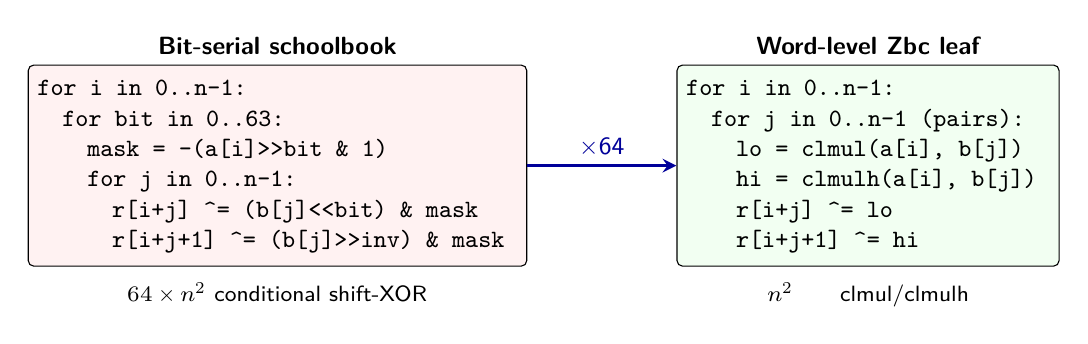
\begin{tikzpicture}[
  box/.style={draw, rounded corners=2pt, minimum width=4.8cm,
    minimum height=2.2cm, align=left, font=\ttfamily\small},
  arrow/.style={->, thick, >=stealth},
  label/.style={font=\sffamily\small\bfseries, above}
]

% Left box: bit-serial schoolbook
\node[box, fill=red!5] (school) at (0,0) {%
  \begin{tabular}{@{}l@{}}
  for i in 0..n-1:\\
  \quad for bit in 0..63:\\
  \quad\quad mask = -(a[i]>>bit \& 1)\\
  \quad\quad for j in 0..n-1:\\
  \quad\quad\quad r[i+j] \^{}= (b[j]<<bit) \& mask\\
  \quad\quad\quad r[i+j+1] \^{}= (b[j]>>inv) \& mask
  \end{tabular}
};
\node[label] at (school.north) {Bit-serial schoolbook};
\node[font=\sffamily\footnotesize, below=2pt] at (school.south)
  {$64 \times n^2$ conditional shift-XOR};

% Right box: clmul leaf
\node[box, fill=green!5] (clmul) at (7.5,0) {%
  \begin{tabular}{@{}l@{}}
  for i in 0..n-1:\\
  \quad for j in 0..n-1 (pairs):\\
  \quad\quad lo = clmul(a[i], b[j])\\
  \quad\quad hi = clmulh(a[i], b[j])\\
  \quad\quad r[i+j] \^{}= lo\\
  \quad\quad r[i+j+1] \^{}= hi
  \end{tabular}
};
\node[label] at (clmul.north) {Word-level \textsf{Zbc} leaf};
\node[font=\sffamily\footnotesize, below=2pt] at (clmul.south)
  {$n^2$ ζεύγη clmul/clmulh};

% Arrow between
\draw[arrow, very thick, color=blue!60!black]
  (school.east) -- node[above, font=\sffamily\small] {$\times$64}
  (clmul.west);

\end{tikzpicture}
}\\[0.6em]
    {\small \pos{\speedup{38.61} \instret} στο \en{leaf kernel} vs \en{bit-serial} (\HQC-128)}
  \end{center}
  \vfill
  \pdfpcnote{budget ≈75s | exit ≈6:40}
  \pdfpcnote{}
  \pdfpcnote{- bit-serial: 64 iter/word, predicated shift-XOR του b[j] στο r[i+j], ακριβο}
  \pdfpcnote{- clmul/clmulh: τα δυο μερη r[i+j], r[i+j+1] απευθειας, χωρις βροχο}
  \pdfpcnote{- figure: αριστερα μασκα ανα bit (XOR σε low/high), δεξια clmul/clmulh μαζι}
  \pdfpcnote{- so-what: ο βροχος 64-bit εξαφανιζεται, >x38 στο leaf}
  \pdfpcnote{}
  \pdfpcnote{cut: λεπτομερεια μασκας, πες μονο "loop -> 1 instruction"}
\end{frame}

\begin{frame}[fragile]{Tier 1: \en{pre-build generator} + \en{assign-on-first-write}}
  \begin{itemize}
    \item \HL{\en{Static code generator}}: σταθερό $N$ $\Rightarrow$ δέντρο αναδρομής γνωστό σε \en{compile time}, πλήρως ξεδιπλωμένο, χωρίς \en{runtime branching}  \end{itemize}
  \vspace{0.2em}
  \begin{center}
    \adjustbox{max width=0.82\linewidth,max totalheight=0.30\textheight,center}{% AP-2 Generator Pipeline diagram
% Used in §6.2.3 (ssec:ap2-generator)

\tikzsetnextfilename{ch6-polymul-ap2-pipeline}
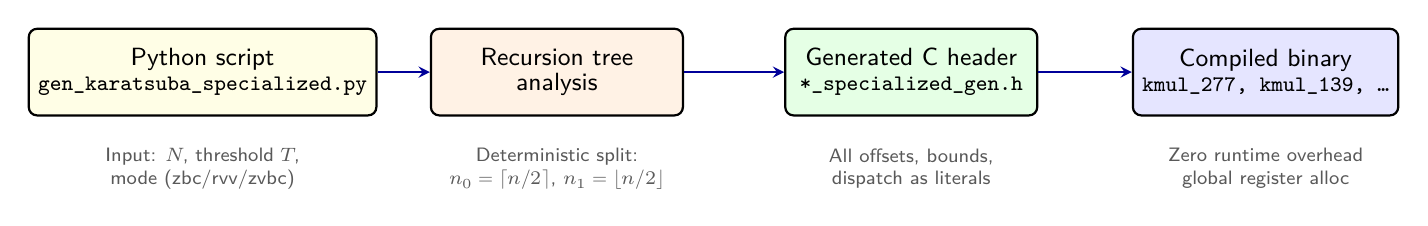
\begin{tikzpicture}[
  stage/.style={draw, rounded corners=3pt, minimum width=3.2cm,
    minimum height=1.1cm, align=center, font=\sffamily\small, thick},
  arrow/.style={->, thick, >=stealth, color=blue!60!black},
  note/.style={font=\sffamily\scriptsize, text=gray!70!black, align=center}
]

% Stage 1: Python script
\node[stage, fill=yellow!10] (script) at (0,0)
  {Python script\\[-2pt]\texttt{\footnotesize gen\_karatsuba\_specialized.py}};

% Stage 2: Recursion tree analysis
\node[stage, fill=orange!10] (tree) at (4.5,0)
  {Recursion tree\\[-2pt]analysis};

% Stage 3: Generated C header
\node[stage, fill=green!10] (header) at (9,0)
  {Generated C header\\[-2pt]\texttt{\footnotesize *\_specialized\_gen.h}};

% Stage 4: Compiled binary
\node[stage, fill=blue!10] (binary) at (13.5,0)
  {Compiled binary\\[-2pt]\texttt{\footnotesize kmul\_277, kmul\_139, \ldots}};

% Arrows
\draw[arrow] (script) -- (tree);
\draw[arrow] (tree) -- (header);
\draw[arrow] (header) -- (binary);

% Annotations below
\node[note, below=8pt] at (script.south) {Input: $N$, threshold $T$,\\mode (zbc/rvv/zvbc)};
\node[note, below=8pt] at (tree.south) {Deterministic split:\\$n_0 = \lceil n/2 \rceil$, $n_1 = \lfloor n/2 \rfloor$};
\node[note, below=8pt] at (header.south) {All offsets, bounds,\\dispatch as literals};
\node[note, below=8pt] at (binary.south) {Zero runtime overhead\\global register alloc};

\end{tikzpicture}
}
  \end{center}
  \vspace{0.2em}
  {\color{accent!40}\rule{\linewidth}{0.6pt}}
  \vspace{0.2em}
  \begin{itemize}
    \item \HL{\en{Assign-on-first-write}}: χωρίς μηδενισμό \en{buffer} ($0 \oplus x = x$)
  \end{itemize}
  \vspace{0.2em}
  \begin{block}{Αποτέλεσμα}
    Σωρευτικά \HL{\speedup{101.3}} \instret σε isolated polymul benchmark (\HQC-128, Tier 1).
  \end{block}
  \pdfpcnote{budget ≈90s | exit ≈8:10}
  \pdfpcnote{}
  \pdfpcnote{- N σταθερο ανα level (277/561/901), δεντρο Karatsuba πληρως προκαθορισμενο}
  \pdfpcnote{- pre-build generator: μια C συναρτηση ανα κομβο, splits/threshold ως σταθερες}
  \pdfpcnote{- ενας generator, τρια backends (zbc/rvv/zvbc), εδω η βαθμωτη Zbc διαδρομη}
  \pdfpcnote{- compiler: full unrolling + constant propagation, μηδεν runtime checks}
  \pdfpcnote{- assign-on-first-write: 0 XOR x = x εξαλειφει το memset}
  \pdfpcnote{- so-what: σωρευτικα x101.3 μονο με Zbc}
  \pdfpcnote{}
  \pdfpcnote{cut: το multi-backend, παε κατευθειαν στο αποτελεσμα}
\end{frame}

% VARIANT of sections/07-vector.tex (frame 1) — L: κάθετη ροή (stacked bullets).
% Υπόθεση: αντικαθιστά το κάτω two-column split με ενιαία κάθετη ροή
% (πρώτα η σημείωση VLMAX, μετά η "Επίδραση στον πυρήνα") και προσθέτει
% οπτικό separator ανάμεσα στο Tier 2 (setup) και στο Tier 3 (λύση στο leaf).
\begin{frame}{Tier 2+3: Διανυσματοποίηση βρόχων ανασύνθεσης και leaf}
  \pdfpcnote{budget ≈75s}
  % --- Tier 2: τι έμεινε ---
  \begin{itemize}
    \item \textbf{Tier 2:} διανυσματοποιεί το \BigO{n} (ανασύνθεση), όχι το \BigO{n^2} leaf
  \end{itemize}
  \vspace{0.3em}
  {\color{gray!45}\hrule}
  \vspace{0.6em}
  % --- Tier 3: η λύση στο leaf ---
  \HL{Tier 3: \vclmul{} υπολογίζει πολλαπλά $64\times64$ carry-less γινόμενα.}
  \vspace{0.3em}
  \begin{center}
    \resizebox{0.82\linewidth}{!}{% Fig: scalar Zbc leaf vs vector Zvbc (vclmul.vx) leaf.
% Presentation-oriented companion to schoolbook-vs-clmul.tex, used by
% presentation-v1/sections/07-vector (Tier 1/2 scalar leaf vs Tier 3 vector leaf).
% Semantic colour: left = costly scalar path (figthreat), right = vector
% solution (figsolution); transition arrow = critical path (figedge/accent).
\tikzsetnextfilename{ch6-polymul-leaf-scalar-vs-vclmul}
\begin{tikzpicture}[
  box/.style={draw, rounded corners=2pt, minimum width=5.0cm,
    minimum height=2.2cm, align=left, figT/mono, figLW/base},
  caption/.style={figT/annot, below=2pt},
]

% Left box: scalar Zbc leaf (costly path)
\node[box, fill=figthreatfill, draw=figthreat] (scalar) at (0,0) {%
  \begin{tabular}{@{}l@{}}
  for i in 0..n-1:\\
  \quad for j in 0..n-1:\\
  \quad\quad lo = clmul(a[i], b[j])\\
  \quad\quad hi = clmulh(a[i], b[j])\\
  \quad\quad r[i+j] \^{}= lo\\
  \quad\quad r[i+j+1] \^{}= hi
  \end{tabular}
};
\node[figT/title, above] at (scalar.north) {Scalar \textsf{Zbc} leaf};
\node[caption] at (scalar.south) {$n^2$ scalar clmul/clmulh};

% Right box: vector Zvbc vclmul.vx leaf (solution)
\node[box, fill=figsolutionfill, draw=figsolution] (vector) at (8.0,0) {%
  \begin{tabular}{@{}l@{}}
  for i in 0..n-1:\\
  \quad vb  = b[0..n-1]\\
  \quad vlo = vclmul.vx(vb, a[i])\\
  \quad vhi = vclmulh.vx(vb, a[i])\\
  \quad vr \^{}= combine(vlo, vhi)
  \end{tabular}
};
\node[figT/title, above] at (vector.north) {Vector \textsf{Zvbc} leaf};
\node[caption] at (vector.south) {1 vclmul.vx/vclmulh.vx per $i$ (VLMAX $=T$)};

% Transition arrow (critical path): inner j-loop collapses to one vector op
\draw[figedge/accent]
  (scalar.east) -- node[above, figT/label] {$j$-loop $n\to1$}
  (vector.west);

\end{tikzpicture}
}
  \end{center}
  % src: figures/ch6-polymul/leaf-scalar-vs-vclmul.tex
  \vspace{0.3em}
  \pause
  \begin{itemize}
    \item Σε \VLEN{}=256, \code{LMUL=m4}: \HL{VLMAX $= T = 16$}, αρκεί ένα vector iteration ανά $i$
    \item \textbf{Αποτέλεσμα:} \HL{\speedup{264}} στον πυρήνα πολ/σμού (\HQC-128, Tier 3)
  \end{itemize}
  \pdfpcnote{Tier 2: ο κρίσιμος βρόχος ανασύνθεσης περνά από scalar XOR σε vxor.vv, γραμμικό κόστος. Ο leaf clmul/clmulh (O(n^2)) ήταν ήδη ο κυρίαρχος όρος, όχι κάτι που εμφανίζεται μετά το Tier 2.}
  \pdfpcnote{.vx μορφή: για κάθε i, το scalar a[i] πολλαπλασιάζεται carry-less με ολόκληρο τον πίνακα b[0..n-1]. Σε VLMAX=16=T ο inner j-loop γίνεται μία iteration, μηδενίζοντας τον scalar inner loop.}
  \pdfpcnote{264 = polymul HQC-128 Tier 3 (σωρευτικά vs scalar_ref). Το HQC-256 (x436) πάει στο results slide.}
\end{frame}

\begin{frame}{Μετά την βελτιστοποίηση: \HL{\en{Keccak}} γίνεται το νέο \en{Amdahl} floor (\pct{49.2})}
  \pdfpcnote{budget ≈45s}
  \HL{Ο πολ/σμός (αρχικά ${\approx}$\pct{97}) υποχωρεί σε ${\approx}$\pct{33} (Tier 1) $\to$ ${\approx}$\pct{22} (Tier 3). Κυρίαρχο πλέον το \en{Keccak}.}
  \vspace{0.3em}
  \begin{columns}[T,onlytextwidth]
    \begin{column}{0.5\textwidth}
      \centering
      \resizebox{0.9\linewidth}{!}{\tikzsetnextfilename{ch6-polymul-pie-scalar-zb}
\begin{tikzpicture}[
    every node/.style={font=\sffamily},
]

% --- Palette via canonical component tokens (cross-figure consistency) ---
\colorlet{colMul}{figkPolymul}
\colorlet{colKeccak}{figkKeccak}
\colorlet{colDecode}{figkDecode}
\colorlet{colMem}{figkMisc}
\colorlet{textmain}{black!75}
\colorlet{textsub}{figneutral}

% --- Parameters ---
\def\mainCX{0}
\def\mainCY{0}
\def\outerR{2.8}
\def\innerR{1.7}

% Helper: ring sector (cx, cy, innerR, outerR, startAngle, endAngle, color)
\newcommand{\ringsectorB}[7]{%
    \fill[#7, draw=white, line width=1.2pt]
        ([shift={(#1,#2)}] #5:#3) arc (#5:#6:#3)
        -- ([shift={(#1,#2)}] #6:#4) arc (#6:#5:#4) -- cycle;
}

% MAIN DONUT — scalar_zb (Tier 1) L128 profile (keccak=ref, decode=ref)
% Polymul = 36.8%  → 132.5°
% Keccak  = 26.5%  →  95.4°
% Decode  = 16.2%  →  58.3°
% Other   = 20.5%  →  73.8°
%
% Angles: start=90, clockwise (90 -> -270)
% Polymul:  90.0  -> -42.5
% Keccak: -42.5  -> -137.9
% Decode: -137.9 -> -196.2
% Other:  -196.2 -> -270.0

\ringsectorB{\mainCX}{\mainCY}{\innerR}{\outerR}{90}{-42.5}{colMul}
\ringsectorB{\mainCX}{\mainCY}{\innerR}{\outerR}{-42.5}{-137.9}{colKeccak}
\ringsectorB{\mainCX}{\mainCY}{\innerR}{\outerR}{-137.9}{-196.2}{colDecode}
\ringsectorB{\mainCX}{\mainCY}{\innerR}{\outerR}{-196.2}{-270}{colMem}

% Labels inside sectors
\pgfmathsetmacro{\labelR}{(\innerR + \outerR)/2}

% Polymul label (mid-angle = (90 + (-42.5))/2 = 23.7)
\node[font=\sffamily\bfseries\small, text=white] at
    ([shift={(\mainCX,\mainCY)}] 23.7:\labelR) {36.8\%};

% Keccak label (mid-angle = (-42.5 + (-137.9))/2 = -90.2)
\node[font=\sffamily\bfseries\small, text=white] at
    ([shift={(\mainCX,\mainCY)}] -90.2:\labelR) {26.5\%};

% Decode label (mid-angle = (-137.9 + (-196.2))/2 = -167.1)
\node[font=\sffamily\bfseries\small, text=white] at
    ([shift={(\mainCX,\mainCY)}] -167.1:\labelR) {16.2\%};

% Other label (mid-angle = (-196.2 + (-270))/2 = -233.1)
\node[font=\sffamily\bfseries\small, text=white] at
    ([shift={(\mainCX,\mainCY)}] -233.1:\labelR) {20.5\%};

% Center text
\node[font=\sffamily\bfseries\large, text=textmain] at (\mainCX, \mainCY+0.15)
    {HQC-128};
\node[font=\sffamily\small, text=textsub] at (\mainCX, \mainCY-0.25)
    {Scalar Zb (Tier~1)};

% LEGEND (bottom)
\def\legY{-\outerR-0.9}
\def\legBoxSize{0.25}

\fill[colMul] (-3.0, \legY) rectangle +(\legBoxSize, \legBoxSize);
\node[font=\sffamily\scriptsize, text=textmain, anchor=west] at (-3.0+\legBoxSize+0.1, \legY+0.12)
    {Polymul};

\fill[colKeccak] (-1.2, \legY) rectangle +(\legBoxSize, \legBoxSize);
\node[font=\sffamily\scriptsize, text=textmain, anchor=west] at (-1.2+\legBoxSize+0.1, \legY+0.12)
    {Keccak/Hashing};

\fill[colDecode] (1.2, \legY) rectangle +(\legBoxSize, \legBoxSize);
\node[font=\sffamily\scriptsize, text=textmain, anchor=west] at (1.2+\legBoxSize+0.1, \legY+0.12)
    {Decode};

\fill[colMem] (3.0, \legY) rectangle +(\legBoxSize, \legBoxSize);
\node[font=\sffamily\scriptsize, text=textmain, anchor=west] at (3.0+\legBoxSize+0.1, \legY+0.12)
    {Other};

\end{tikzpicture}
}
    \end{column}
    \begin{column}{0.5\textwidth}
      \centering
      \resizebox{0.9\linewidth}{!}{\tikzsetnextfilename{ch6-polymul-pie-vector-zvk}
\begin{tikzpicture}[
    every node/.style={font=\sffamily},
]

% --- Palette via canonical component tokens (cross-figure consistency) ---
\colorlet{colMul}{figkPolymul}
\colorlet{colKeccak}{figkKeccak}
\colorlet{colDecode}{figkDecode}
\colorlet{colMem}{figkMisc}
\colorlet{textmain}{black!75}
\colorlet{textsub}{figneutral}

% --- Parameters ---
\def\mainCX{0}
\def\mainCY{0}
\def\outerR{2.8}
\def\innerR{1.7}

% Helper: ring sector (cx, cy, innerR, outerR, startAngle, endAngle, color)
\newcommand{\ringsectorC}[7]{%
    \fill[#7, draw=white, line width=1.2pt]
        ([shift={(#1,#2)}] #5:#3) arc (#5:#6:#3)
        -- ([shift={(#1,#2)}] #6:#4) arc (#6:#5:#4) -- cycle;
}

% MAIN DONUT — vector_zvk (Tier 3) L128 profile (keccak=ref, decode=ref)
% Polymul = 21.8%  →  78.5°
% Keccak  = 49.2%  → 177.1°
% Decode  = 24.0%  →  86.4°
% Other   =  5.1%  →  18.4°
%
% Angles: start=90, clockwise (90 -> -270)
% Polymul:  90.0  ->  11.5
% Keccak:  11.5  -> -165.6
% Decode: -165.6  -> -252.0
% Other:  -252.0  -> -270.0

\ringsectorC{\mainCX}{\mainCY}{\innerR}{\outerR}{90}{11.5}{colMul}
\ringsectorC{\mainCX}{\mainCY}{\innerR}{\outerR}{11.5}{-165.6}{colKeccak}
\ringsectorC{\mainCX}{\mainCY}{\innerR}{\outerR}{-165.6}{-252.0}{colDecode}
\ringsectorC{\mainCX}{\mainCY}{\innerR}{\outerR}{-252.0}{-270}{colMem}

% Labels inside sectors
\pgfmathsetmacro{\labelR}{(\innerR + \outerR)/2}

% Polymul label (mid-angle = (90 + 11.5)/2 = 50.8)
\node[font=\sffamily\bfseries\small, text=white] at
    ([shift={(\mainCX,\mainCY)}] 50.8:\labelR) {21.8\%};

% Keccak label (mid-angle = (11.5 + (-165.6))/2 = -77.1)
\node[font=\sffamily\bfseries\small, text=white] at
    ([shift={(\mainCX,\mainCY)}] -77.1:\labelR) {49.2\%};

% Decode label (mid-angle = (-165.6 + (-252.0))/2 = -208.8)
\node[font=\sffamily\bfseries\small, text=white] at
    ([shift={(\mainCX,\mainCY)}] -208.8:\labelR) {24.0\%};

% Other label (mid-angle = (-252.0 + (-270))/2 = -261.0)
\node[font=\sffamily\bfseries\footnotesize, text=white] at
    ([shift={(\mainCX,\mainCY)}] -261.0:\labelR) {5.1\%};

% Center text
\node[font=\sffamily\bfseries\large, text=textmain] at (\mainCX, \mainCY+0.15)
    {HQC-128};
\node[font=\sffamily\small, text=textsub] at (\mainCX, \mainCY-0.25)
    {Vector Zvk (Tier~3)};

% LEGEND (bottom)
\def\legY{-\outerR-0.9}
\def\legBoxSize{0.25}

\fill[colMul] (-3.0, \legY) rectangle +(\legBoxSize, \legBoxSize);
\node[font=\sffamily\scriptsize, text=textmain, anchor=west] at (-3.0+\legBoxSize+0.1, \legY+0.12)
    {Polymul};

\fill[colKeccak] (-1.2, \legY) rectangle +(\legBoxSize, \legBoxSize);
\node[font=\sffamily\scriptsize, text=textmain, anchor=west] at (-1.2+\legBoxSize+0.1, \legY+0.12)
    {Keccak/Hashing};

\fill[colDecode] (1.2, \legY) rectangle +(\legBoxSize, \legBoxSize);
\node[font=\sffamily\scriptsize, text=textmain, anchor=west] at (1.2+\legBoxSize+0.1, \legY+0.12)
    {Decode};

\fill[colMem] (3.0, \legY) rectangle +(\legBoxSize, \legBoxSize);
\node[font=\sffamily\scriptsize, text=textmain, anchor=west] at (3.0+\legBoxSize+0.1, \legY+0.12)
    {Other};

\end{tikzpicture}
}
    \end{column}
  \end{columns}
  % src: figures/ch6-polymul/{pie-scalar-zb,pie-vector-zvk}.tex (HQC-128 instret profile)
  \pdfpcnote{Scalar Zb (Tier 1): polymul 32.7, Keccak 33.7, decode 15.3, other 18.2. Vector Zvk (Tier 3): polymul 21.8, Keccak 49.2, decode 24.0, other 5.1. Αυτό αιτιολογεί γιατί τα επόμενα βήματα στοχεύουν Keccak/decode.}
\end{frame}

% --- 08 Keccak & decode ------------------------------------------------------
\begin{frame}{Οι δύο εναπομείναντες πυρήνες: \en{Keccak} (scalar \Zbb) \& \en{decode} (\RVV)}
  \begin{columns}[T]
    \begin{column}{0.50\textwidth}
      \textbf{\en{Keccak}-$f[1600]$}
      \begin{itemize}\small
        \item \HL{Scalar \Zbb idiom recognition}: \rori, \insn{andn} \enspace$\Rightarrow$\enspace \speedup{1.36}
        \item \con{Παράδοξο RVV}: \en{LMUL=8} \con{πιο αργό} από scalar: \num{4} register groups $\Rightarrow$ \con{spills} $+$ κόστος \insn{vrgather.vv} \con{${\sim}$τετραγωνικό με} \en{LMUL}
        \item \pos{Ουσιαστική λύση}: αφιερωμένη εντολή \en{HW} (\en{RISC-V PQC}, v1.0 στόχος 31/12/2026)
      \end{itemize}
    \end{column}
    \begin{column}{0.50\textwidth}
      \textbf{\en{Reed--Muller/Solomon decode}}
      \begin{itemize}\small
        \item \en{Tier 1} scalar: \code{gf\_mul} $\to$ ένα \clmul
        \item \en{RM} \en{FHT}: διανυσματικά \RVV βήματα
        \item \en{RS} επί του \GF{2^8} με \vclmul (\Zvbc)
        \item Έναντι βαθμωτής \en{ref.} \enspace$\Rightarrow$\enspace \HL{\speedup{14.3}}
      \end{itemize}
    \end{column}
  \end{columns}
  \pdfpcnote{budget 75s}
  \pdfpcnote{}
  \pdfpcnote{- Keccak: το idiom recognition (rori/andn) φτάνει ήδη το βέλτιστο scalar. Vectorization = τεκμηριωμένο αρνητικό αποτέλεσμα, όχι παράλειψη.}
  \pdfpcnote{- LMUL=8 βραδύτερη: 4 μόνο register groups -> spills/γύρο + vrgather.vv ~τετραγωνικό στο LMUL. Δρόμος: αφιερωμένη εντολή HW (ολόκληρη μετάθεση σε μία εντολή).}
  \pdfpcnote{- Q: μεταφορές μία φορά πριν/μετά; Όχι: 4 fused βήματα στενά συζευγμένα, καθένα διαφορετικό cross-lane pattern -> hybrid = per-element μεταφορές μέσα στη ροή. Πλήρως vector = ακριβά shuffles στα ρ/π/χ.}
  \pdfpcnote{- Decode: x14.3 = RM (FHT/RVV) + RS (Zvbc). Αν ρωτηθώ, backup με ανάλυση ανά βήμα.}
  \pdfpcnote{}
  \pdfpcnote{cut: αν καθυστερώ, μόνο τα δύο headline (x1.36, x14.3).}
\end{frame}


\section{Πειραματικά Αποτελέσματα}
% --- 09 Experimental setup ---------------------------------------------------
\begin{frame}{Πειραματική διάταξη: τριπλή επαλήθευση}
  \begin{columns}[T,onlytextwidth]
    \begin{column}{0.62\textwidth}
      \begin{itemize}
        \item \HL{\en{Spike ISS}}: μέτρηση \instret (αρχιτεκτονικά ανεξάρτητη) — όλες οι βαθμίδες
        \item \HL{\en{QEMU}}: επικύρωση ορθότητας μέσω \en{KAT} (\en{known-answer tests})
        \item \HL{\en{Banana Pi BPI-F3}} (\en{SpacemiT K1}, πυρήνας X60, $\VLEN=256$): πραγματικοί κύκλοι ρολογιού
      \end{itemize}
      \vspace{0.4em}
      \begin{block}{Γιατί \instret;}
        Αποσυνδέει την αλγοριθμική βελτίωση από το μικροαρχιτεκτονικό θόρυβο — αναπαραγώσιμη, συγκρίσιμη μετρική.
      \end{block}
    \end{column}
    \begin{column}{0.38\textwidth}
      \begin{exampleblock}{Συνέπεια}
        Στις βαθμίδες που τρέχουν σε πραγματικό υλικό (1--2), η απόκλιση \instret ↔ κύκλοι είναι \HL{$\sim\!\pct{2}$}.
      \end{exampleblock}
    \end{column}
  \end{columns}
\end{frame}

% --- 10 Results (HEADLINE) ---------------------------------------------------
% Provenance: results/reports/summaries/speedups_simulation.md (Spike instret, VLEN=256, specialized tree).
% KEM end-to-end speedups vs HQC reference implementation.
\begin{frame}{Αποτελέσματα: επιτάχυνση end-to-end \KEM}
  \begin{columns}[c,onlytextwidth]
    \begin{column}{0.46\textwidth}
      \renewcommand{\arraystretch}{1.25}
      \begin{tabular}{@{}lcc@{}}
        \toprule
        Βαθμίδα & \HQC-128 & \HQC-256 \\
        \midrule
        1 · σειριακή (\Zbc) & \speedup{34.0} & \speedup{49.1} \\
        2 · \RVV          & \speedup{60.0} & \speedup{71.7} \\
        3 · \en{vec-crypto} & \HL{\speedup{167.0}} & \HL{\speedup{338.8}} \\
        \bottomrule
      \end{tabular}\\[0.6em]
      {\footnotesize Πυρήνας πολ/σμού (Βαθμίδα 3): \HL{\speedup{318}} / \HL{\speedup{547}}}
    \end{column}
    \begin{column}{0.54\textwidth}
      \centering
      \tikzsetnextfilename{pres-results-kem-bars}
      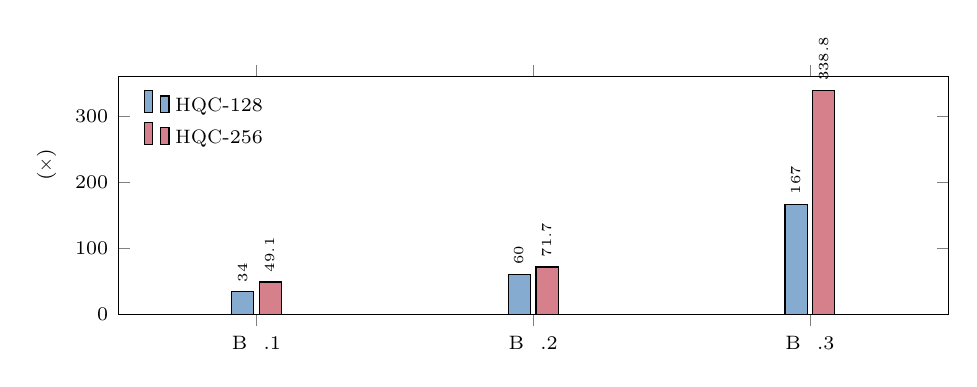
\begin{tikzpicture}
        \begin{axis}[
            ybar, width=\textwidth, height=4.6cm,
            bar width=8pt, enlarge x limits=0.25,
            ymin=0, ymax=360,
            ylabel={\scriptsize επιτάχυνση ($\times$)},
            symbolic x coords={Βαθμ.1,Βαθμ.2,Βαθμ.3},
            xtick=data, x tick label style={font=\scriptsize},
            ytick={0,100,200,300}, y tick label style={font=\scriptsize},
            legend style={font=\scriptsize,at={(0.02,0.97)},anchor=north west,draw=none},
            nodes near coords, every node near coord/.append style={font=\tiny,rotate=90,anchor=west},
        ]
          \addplot[fill=hlc!55] coordinates {(Βαθμ.1,34.0) (Βαθμ.2,60.0) (Βαθμ.3,167.0)};
          \addplot[fill=conc!55] coordinates {(Βαθμ.1,49.1) (Βαθμ.2,71.7) (Βαθμ.3,338.8)};
          \legend{\HQC-128,\HQC-256}
        \end{axis}
      \end{tikzpicture}\\
      {\footnotesize Έναντι αναφορικής υλοποίησης \HQC · \en{Spike} \instret}
    \end{column}
  \end{columns}
  \vspace{0.2em}
  \pause
  \begin{exampleblock}{}
    \centering Κλιμάκωση με το security level: όσο μεγαλύτερα τα πολυώνυμα, \HL{τόσο μεγαλύτερο το όφελος} του διανυσματικού πολ/σμού.
  \end{exampleblock}
\end{frame}

% VARIANT — not \input by main.tex; promote with promote-slide.sh
% Variant of 11-hardware.tex — LAYOUT (L=_bigfact) + INFORMATION-SCOPE (I):
%   δύο κυρίαρχα big-fact ratio (regime dichotomy)· absolute speedups demoted/dropped.
% Data/provenance unchanged: chapters/08-results.tex :: tab:hw-spike-prediction-levels
\begin{frame}{Το \instret προβλέπει \pos{αξιόπιστα} το scalar, \con{αισιόδοξα} το vector}
  \vspace{0.4em}
  \begin{columns}[T,onlytextwidth]
    \begin{column}{0.5\textwidth}
      \centering
      {\large\pos{\textbf{Βαθμωτά (Tier~1)}}}\\[0.3em]
      {\Huge\pos{\num{1.07}--\num{1.10}}}\\[0.2em]
      {\footnotesize λόγος \en{HW/Spike}}\\[0.6em]
      \pos{\en{HW} $>$ πρόβλεψη}\\ \small \en{dual-issue}, \en{IPC}$>$1
    \end{column}
    \begin{column}{0.5\textwidth}
      \centering
      {\large\con{\textbf{Διανυσματικά (Tier~2)}}}\\[0.3em]
      {\Huge\con{\num{0.82}--\num{0.90}}}\\[0.2em]
      {\footnotesize λόγος \en{HW/Spike}}\\[0.6em]
      \con{\en{HW} $<$ πρόβλεψη}\\ \small scalar$\leftrightarrow$vector penalties
    \end{column}
  \end{columns}
  \vspace{0.8em}
  \begin{center}\footnotesize
    Πλήρες \KEM, \en{BPI-F3} (\en{SpacemiT X60}, \en{VLEN}$=$256).
  \end{center}
  \pdfpcnote{Bigfact variant: δυο καθεστωτα. Scalar 1.07-1.10 (HW ξεπερνα). Vector 0.82-0.90 (Spike overpredicts, penalties). Οι absolute speedups ειναι στο table/fulldata variant.}
\end{frame}
% --- 12 Comparison with related work -----------------------------------------
% Provenance: figures/ch9-discussion/cross-architecture-table.tex (trimmed).
\begin{frame}{Σύγκριση με σχετικές εργασίες}
  \centering
  \renewcommand{\arraystretch}{1.2}
  {\small
  \begin{tabular}{@{}llll@{}}
    \toprule
    Εργασία & Πλατφόρμα & Προσέγγιση & Επιτάχυνση \\
    \midrule
    \en{Sch\"offel}~\cite{Schoeffel2022-HQC-IoT} & RV32 (SW) & καθαρό λογισμικό & — (baseline) \\
    \en{FAFFT}~\cite{OptHQC2025} & RV32 + \en{FPGA} & καθαρό λογισμικό & χαμηλή \\
    \en{pqm4}~\cite{Jang2025-CortexM4-HQC} & ARM Cortex-M4 & bit-slicing & μέτρια \\
    \midrule
    \HL{Παρούσα εργασία} & RV64GC + κρυπτο-\en{ISA} & \HL{εγγενείς εντολές} & \HL{έως \speedup{339}} \\
    \bottomrule
  \end{tabular}}
  \vspace{0.6em}
  \begin{itemize}
    \item Οι προηγούμενες RISC-V εργασίες είναι \con{καθαρά λογισμικές} ή απαιτούν custom \en{FPGA}
    \item \HL{Πρώτη εργασία} που αξιοποιεί \HL{επικυρωμένες κρυπτογραφικές επεκτάσεις} για το \HQC
  \end{itemize}
  \vspace{-0.2em}
  {\footnotesize Πλήρης πίνακας κύκλων/\instret στο παράρτημα.}
\end{frame}


\section{Συμπεράσματα}
% --- 13 Conclusions, limitations & future work -------------------------------
\begin{frame}{Συμπεράσματα, περιορισμοί \& μελλοντική εργασία}
  \textbf{Συμπεράσματα}
  \begin{enumerate}
    \item \HL{Πρώτη πλήρης υλοποίηση του \HQC σε RISC-V} με επεκτάσεις \en{ISA}
    \item Επιτάχυνση \KEM \HL{\speedup{76}} (\HQC-128) έως \HL{\speedup{164}} (\HQC-256) σε \instret
  \end{enumerate}
  \vspace{0.8em}
  {\color{gray!45}\hrule}
  \vspace{1.5em}
  \pause
  \begin{columns}[T,onlytextwidth]
    \begin{column}{0.5\textwidth}
      \textbf{Περιορισμοί}
      \begin{itemize}
        \item Tier 3 (\Zvbc/\Zvbb): μόνο σε Spike, όχι μετρήσεις σε κύκλους
        \item \en{Keccak floor}: άνω όριο χωρίς την εντολή \code{vkeccak.vi}
      \end{itemize}
    \end{column}
    \begin{column}{0.5\textwidth}
      \textbf{Μελλοντική εργασία}
      \begin{itemize}
        \item Tier~3 σε \en{hardware}: \en{SpacemiT K3} (\Zvbc, Μάιος 2026)
        \item Ενσωμάτωση \code{vkeccak.vi} (\en{RVS-2360})
      \end{itemize}
    \end{column}
  \end{columns}
\end{frame}

% --- 14 Limitations & future work --------------------------------------------
\begin{frame}{Περιορισμοί \& μελλοντική εργασία}
  \begin{columns}[T,onlytextwidth]
    \begin{column}{0.5\textwidth}
      \textbf{Περιορισμοί}
      \begin{itemize}
        \item Βαθμίδα 3 (\Zvbc/\Zvbb): μόνο σε εξομοίωση, δεν υπάρχει ακόμη παραγωγικό \en{silicon}
        \item Τα αποτελέσματα βαθμίδας 3 είναι σε \instret, όχι κύκλους
        \ifincludeCT\item Η \en{constant-time} επαλήθευση είναι εμπειρική (όχι τυπική απόδειξη)\fi
      \end{itemize}
    \end{column}
    \begin{column}{0.5\textwidth}
      \textbf{Μελλοντική εργασία}
      \begin{itemize}
        \item Μετρήσεις κύκλων σε μελλοντικό \en{vector-crypto} υλικό
        \ifincludeCT\item Τυπική απόδειξη \en{constant-time} (formal CT)\fi
        \item Επέκταση σε άλλα \en{code-based} σχήματα (\en{BIKE}, \en{Classic McEliece})
      \end{itemize}
    \end{column}
  \end{columns}
\end{frame}

% --- 15 Thanks / questions ---------------------------------------------------
{
\setbeamercolor{background canvas}{bg=accent}
\begin{frame}[plain]
  \centering
  \vfill
  {\color{white}\Huge Ευχαριστώ!}\\[0.8em]
  {\color{white}\large Ερωτήσεις;}\\[1.2em]
  {\color{white}\footnotesize Φραϊδάκης Ιωάννης · \en{\texttt{github.com/fraidakis/hqc-riscv-thesis}}}
  \vfill
\end{frame}
}


% --- Backup (after the closing frame; not counted in the 15') ----------------
\appendix
% =============================================================================
% backup.tex — appendix frames (answers to anticipated committee questions)
% Not counted in the 15'. All numbers traceable to results/reports/ & figures/.
% =============================================================================
\begin{frame}{Παράρτημα: διαδικασία τυποποίησης NIST (2016--2025)}
  \centering
  \resizebox{0.9\linewidth}{!}{% VARIANT — not \input by main.tex; promote manually.
% _v1 — beautified original + TOKEN MIGRATION of nist-rounds-flowchart.tex.
% Same vertical top-to-bottom layout & data; local glyph/leader/box styles
% migrated to thesis-tikz-styles.tex tokens. FIX: the original used an UNDEFINED
% `figleader' style for the axis-to-box leaders (no such token in the style
% file) — replaced here with the hairline `figrule, figLW/hair'. The deepening
% process tint (roundbox=#1) is an intentional gradient, kept.
\tikzsetnextfilename{ch1-introduction-nist-rounds-flowchart_v1}
\begin{tikzpicture}[
  vbox/.style={
    draw=figrule, rounded corners=2pt, text width=8.2cm, align=left,
    inner sep=6pt, figT/label, anchor=west
  },
  roundbox/.style={vbox, fill=figprocess!#1},
  milestonebox/.style={vbox, draw=figsolution, figLW/base, fill=figsolutionfill},
  hqcbox/.style={vbox, draw=figaccent, figLW/emph, fill=figaccentfill},
  yr/.style={font=\sffamily\scriptsize\bfseries, text=figneutral, anchor=east},
]
\def\bx{1.3}

% --- Vertical axis ---
\draw[figrule, figLW/emph] (0,0.7) -- (0,-13.0);
\draw[figrule, figLW/emph, -{Stealth[length=5pt]}] (0,-13.0) -- (0,-13.4);

% --- Leader from axis to each box (FIX: was undefined figleader) ---
\foreach \y in {0,-2,-4,-6,-8,-10,-12} { \draw[figrule, figLW/hair] (0,\y) -- (\bx,\y); }

% === Rounds (process, deepening cool tint) ===
\node[figglyph/event] at (0,0) {}; \node[yr] at (-0.18,0) {2016};
\node[roundbox=12, anchor=west] at (\bx,0) {%
  {\sffamily\bfseries\color{figprocess!80!black} Πρόσκληση Υποβολών}\\[1pt]
  Ανοιχτή διαδικασία τυποποίησης PQC· 82 υποβολές $\to$ 69 δεκτοί υποψήφιοι.%
};
\node[figglyph/event] at (0,-2) {}; \node[yr] at (-0.18,-2) {2017};
\node[roundbox=20, anchor=west] at (\bx,-2) {%
  {\sffamily\bfseries\color{figprocess!80!black} Γύρος 1 · Αρχική Αξιολόγηση}\\[1pt]
  Δημόσια κρυπτανάλυση των υποψηφίων· 69 $\to$ 26 για τον Γύρο 2.%
};
\node[figglyph/event] at (0,-4) {}; \node[yr] at (-0.18,-4) {2019};
\node[roundbox=30, anchor=west] at (\bx,-4) {%
  {\sffamily\bfseries\color{figprocess!80!black} Γύρος 2 · Αξιολόγηση Απόδοσης}\\[1pt]
  Απόδοση \& ασφάλεια· 26 $\to$ 7 finalists + 8 alternates.%
};
\node[figglyph/event] at (0,-6) {}; \node[yr] at (-0.18,-6) {2020};
\node[roundbox=40, anchor=west] at (\bx,-6) {%
  {\sffamily\bfseries\color{figprocess!85!black} Γύρος 3 · Τελικοί Υποψήφιοι}\\[1pt]
  7+8 υποψήφιοι $\to$ 4 προς τυποποίηση + 4 KEMs στον Γύρο 4.%
};
\node[figglyph/event] at (0,-8) {}; \node[yr] at (-0.18,-8) {2022};
\node[roundbox=50, anchor=west] at (\bx,-8) {%
  {\sffamily\bfseries\color{figprocess!90!black} Γύρος 4 · Μη-Lattice KEM}\\[1pt]
  Τέσσερις υποψήφιοι: BIKE, Classic McEliece, \HQC, SIKE.%
};

% === Milestones (solution / accent) ===
\node[figglyph/standard] at (0,-10) {}; \node[yr] at (-0.18,-10) {2024};
\node[milestonebox, anchor=west] at (\bx,-10) {%
  {\sffamily\bfseries\color{figsolution!55!black} Πρώτα Πρότυπα FIPS}\\[1pt]
  FIPS 203 (ML-KEM), 204 (ML-DSA), 205 (SLH-DSA) — lattice \& hash-based.%
};
\node[figglyph/focal] at (0,-12) {}; \node[yr] at (-0.18,-12) {2025};
\node[hqcbox, anchor=west] at (\bx,-12) {%
  {\sffamily\bfseries\color{figaccent} Επιλογή \HQC · Μάρτιος 2025}\\[1pt]
  Πέμπτο PQC πρότυπο· draft FIPS 2026, τελικό πρότυπο 2027.%
};

\end{tikzpicture}
}
  % src: figures/ch1-introduction/nist-rounds-flowchart.tex
\end{frame}

\begin{frame}{Παράρτημα: παράμετροι \HQC}
  \centering
  \renewcommand{\arraystretch}{1.2}
  {\small
  \begin{tabular}{@{}lrrrr@{}}
    \toprule
    Επίπεδο & $N$ & $n_1$ & $n_2$ & $\omega$ \\
    \midrule
    \HQC-128 & \num{17669} & 46 & 384 & 66 \\
    \HQC-192 & \num{35851} & 56 & 640 & 100 \\
    \HQC-256 & \num{57637} & 90 & 640 & 131 \\
    \bottomrule
  \end{tabular}}
  % src: figures/ch2-background/hqc-params-table.tex
  \par\medskip
  \begin{minipage}{0.86\textwidth}
    \begin{itemize}
      \item $N$ : διάσταση δακτυλίου (μέγιστος βαθμός πολυωνύμου)
      \item $n_1$ : μήκος \en{RS} codeword (σύμβολα)
      \item $n_2$ : μήκος \en{RM} codeword (bits)
      \item $\omega$ : βάρος \en{Hamming} μυστικού
    \end{itemize}
  \end{minipage}
\end{frame}

\begin{frame}{Παράρτημα: \en{Keccak} (sponge \& state) και οι πράξεις \Zbb}
  \begin{columns}[T,onlytextwidth]
    \begin{column}{0.50\textwidth}
      \resizebox{\linewidth}{!}{% Sponge construction diagram for SHA-3/Keccak
% Shows absorb phase (XOR + permute) and squeeze phase (extract + permute)
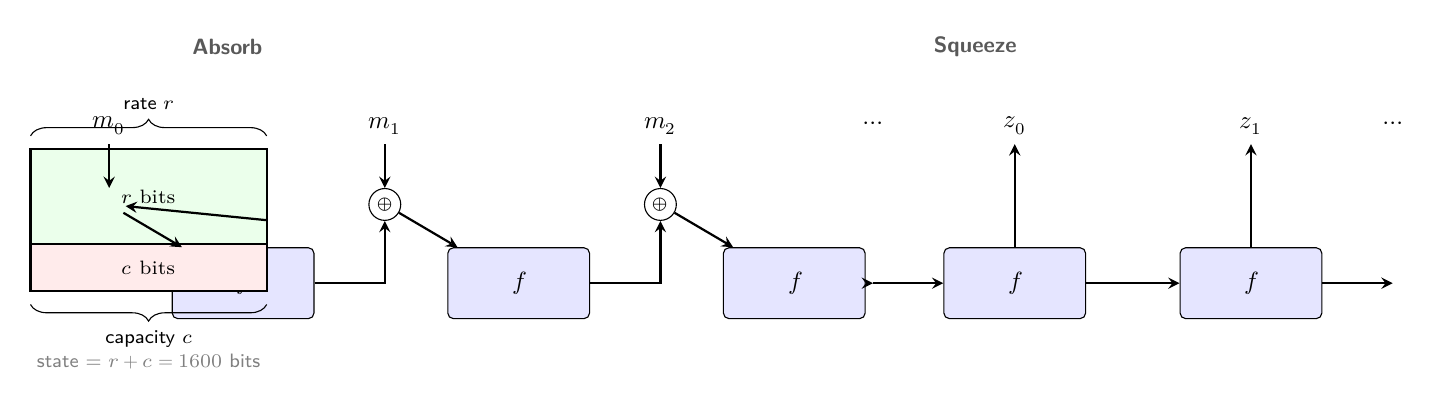
\begin{tikzpicture}[
  >=stealth,
  block/.style={draw, minimum width=1.8cm, minimum height=0.9cm,
                font=\small\sffamily, align=center, rounded corners=2pt},
  xornode/.style={draw, circle, inner sep=1.5pt, font=\scriptsize},
  arr/.style={->, thick},
  brace/.style={decorate, decoration={brace, amplitude=6pt, raise=2pt}},
  label/.style={font=\footnotesize\sffamily, text=gray!70!black}
]

% State representation
\def\stateW{3.0}
\def\rateH{1.2}
\def\capH{0.6}

% --- Absorb phase ---
\node[label] at (0, 2.5) {\textbf{Absorb}};

% Input blocks
\node[font=\small] (m0) at (-1.5, 1.5) {$m_0$};
\node[font=\small] (m1) at (2.0, 1.5) {$m_1$};
\node[font=\small] (m2) at (5.5, 1.5) {$m_2$};
\node[font=\small] (dots) at (8.2, 1.5) {$\cdots$};

% XOR nodes
\node[xornode] (xor0) at (-1.5, 0.5) {$\oplus$};
\node[xornode] (xor1) at (2.0, 0.5) {$\oplus$};
\node[xornode] (xor2) at (5.5, 0.5) {$\oplus$};

% Permutation blocks
\node[block, fill=blue!10] (f0) at (0.2, -0.5) {$f$};
\node[block, fill=blue!10] (f1) at (3.7, -0.5) {$f$};
\node[block, fill=blue!10] (f2) at (7.2, -0.5) {$f$};

% State boxes (rate + capacity)
\draw[thick, fill=green!8] (-2.5, 0.0) rectangle (-2.5+\stateW, \rateH);
\node[font=\scriptsize] at (-2.5+\stateW/2, \rateH/2) {$r$ bits};
\draw[thick, fill=red!8] (-2.5, -\capH) rectangle (-2.5+\stateW, 0.0);
\node[font=\scriptsize] at (-2.5+\stateW/2, -\capH/2) {$c$ bits};

% Arrows: input to XOR
\draw[arr] (m0) -- (xor0);
\draw[arr] (m1) -- (xor1);
\draw[arr] (m2) -- (xor2);

% Arrows: XOR to f
\draw[arr] (xor0) -- (f0);
\draw[arr] (xor1) -- (f1);
\draw[arr] (xor2) -- (f2);

% Arrows: f to next XOR
\draw[arr] (f0) -| (xor1);
\draw[arr] (f1) -| (xor2);
\draw[arr] (f2) -- (8.2, -0.5);

% Initial state arrow
\draw[arr] (-2.5+\stateW, 0.3) -- (xor0);

% --- Squeeze phase ---
\node[label] at (9.5, 2.5) {\textbf{Squeeze}};

\node[block, fill=blue!10] (fs0) at (10.0, -0.5) {$f$};
\node[block, fill=blue!10] (fs1) at (13.0, -0.5) {$f$};

% Output blocks
\node[font=\small] (z0) at (10.0, 1.5) {$z_0$};
\node[font=\small] (z1) at (13.0, 1.5) {$z_1$};
\node[font=\small] (zdots) at (14.8, 1.5) {$\cdots$};

% Arrows: f to output
\draw[arr] (fs0) -- (z0);
\draw[arr] (fs1) -- (z1);

% Arrows: chain
\draw[arr] (8.2, -0.5) -- (fs0);
\draw[arr] (fs0) -- (fs1);
\draw[arr] (fs1) -- (14.8, -0.5);

% Rate/capacity annotation
\draw[brace] (-2.5, \rateH+0.1) -- node[above=8pt, font=\scriptsize\sffamily]
  {rate $r$} (-2.5+\stateW, \rateH+0.1);
\draw[brace] (-2.5+\stateW, -\capH-0.1) -- node[below=8pt, font=\scriptsize\sffamily]
  {capacity $c$} (-2.5, -\capH-0.1);

% Annotation: state width
\node[font=\scriptsize\sffamily, text=gray] at (-1.0, -1.5)
  {state = $r + c = \num{1600}$ bits};

\end{tikzpicture}
}
    \end{column}
    \begin{column}{0.04\textwidth}
      \centering
      {\tikzexternaldisable
       \begin{tikzpicture}
         \draw[dashed, gray!60, line width=0.6pt] (0,0) -- (0,3.8);
       \end{tikzpicture}}
    \end{column}
    \begin{column}{0.42\textwidth}
      \resizebox{\linewidth}{!}{\tikzsetnextfilename{ch2-background-keccak-state-3d}
\begin{tikzpicture}[
  x={(0.9cm, 0cm)}, y={(0.35cm, 0.35cm)}, z={(0cm, 0.8cm)},
  font=\sffamily\small
]

\def\cellsize{0.8}
\def\depth{2.5}

% Bottom face grid
\foreach \x in {0,...,4} {
  \foreach \y in {0,...,4} {
    \draw[figLW/hair, draw=figrule, fill=black!4, fill opacity=0.5]
      (\x*\cellsize, \y*\cellsize, 0) --
      (\x*\cellsize+\cellsize, \y*\cellsize, 0) --
      (\x*\cellsize+\cellsize, \y*\cellsize+\cellsize, 0) --
      (\x*\cellsize, \y*\cellsize+\cellsize, 0) -- cycle;
  }
}

% Lane highlight (x=1, y=2) — figaccent (three visible faces)
\fill[figaccent, opacity=0.35]
  (1*\cellsize, 2*\cellsize, 0) -- (1*\cellsize+\cellsize, 2*\cellsize, 0) --
  (1*\cellsize+\cellsize, 2*\cellsize, \depth) -- (1*\cellsize, 2*\cellsize, \depth) -- cycle;
\fill[figaccent, opacity=0.25]
  (1*\cellsize, 2*\cellsize, 0) -- (1*\cellsize, 2*\cellsize+\cellsize, 0) --
  (1*\cellsize, 2*\cellsize+\cellsize, \depth) -- (1*\cellsize, 2*\cellsize, \depth) -- cycle;
\fill[figaccent, opacity=0.45]
  (1*\cellsize, 2*\cellsize, \depth) -- (1*\cellsize+\cellsize, 2*\cellsize, \depth) --
  (1*\cellsize+\cellsize, 2*\cellsize+\cellsize, \depth) -- (1*\cellsize, 2*\cellsize+\cellsize, \depth) -- cycle;

% Column highlight (x=3, all y) — figsolution
\foreach \y in {0,...,4} {
  \fill[figsolution, opacity=0.30]
    (3*\cellsize, \y*\cellsize, 0) -- (3*\cellsize+\cellsize, \y*\cellsize, 0) --
    (3*\cellsize+\cellsize, \y*\cellsize+\cellsize, 0) -- (3*\cellsize, \y*\cellsize+\cellsize, 0) -- cycle;
}

% Vertical depth edges
\foreach \x in {0,4} {
  \foreach \y in {0,4} {
    \draw[figLW/hair, draw=figrule] (\x*\cellsize, \y*\cellsize, 0) -- (\x*\cellsize, \y*\cellsize, \depth);
  }
}
\draw[figLW/hair, draw=figrule] (5*\cellsize, 0, 0) -- (5*\cellsize, 0, \depth);
\draw[figLW/hair, draw=figrule] (5*\cellsize, 5*\cellsize, 0) -- (5*\cellsize, 5*\cellsize, \depth);
\draw[figLW/hair, draw=figrule] (0, 5*\cellsize, 0) -- (0, 5*\cellsize, \depth);

% Top face outline
\draw[figLW/hair, draw=figrule]
  (0, 0, \depth) -- (5*\cellsize, 0, \depth) --
  (5*\cellsize, 5*\cellsize, \depth) -- (0, 5*\cellsize, \depth) -- cycle;

% Axis labels
\draw[figLW/base, draw=figneutral, <->] (-0.5, 0, 0) -- (-0.5, 5*\cellsize, 0)
  node[midway, left, figT/micro] {$y$ (5)};
\draw[figLW/base, draw=figneutral, <->] (0, -0.5, 0) -- (5*\cellsize, -0.5, 0)
  node[midway, below, figT/micro] {$x$ (5)};
\draw[figLW/base, draw=figneutral, <->] (5*\cellsize+0.5, 0, 0) -- (5*\cellsize+0.5, 0, \depth)
  node[midway, right, figT/micro] {$z$ (64 bits)};

% Annotations
\node[figT/micro, text=figaccent!70!black, anchor=west] at (6, 2.5*\cellsize, 1.2)
  {Lane $A[x,y]$};
\draw[figLW/hair, draw=figaccent!70!black, ->] (6, 2.5*\cellsize, 1.2) -- (1.5*\cellsize, 2.5*\cellsize, 1.2);

\node[figT/micro, text=figsolution!60!black, anchor=west] at (6, 0.5*\cellsize, 0)
  {Column $A[x,*,z]$};
\draw[figLW/hair, draw=figsolution!60!black, ->] (6, 0.5*\cellsize, 0) -- (3.5*\cellsize, 2*\cellsize, 0);

% Title annotation — dropped straight down (negative z) for clear separation from the figure
\node[figT/annot, anchor=north] at (2.8*\cellsize, 0, -1.0)
  {Κατάσταση Keccak: $5 \times 5 \times 64 = \num{1600}$ bits};

\end{tikzpicture}
}
    \end{column}
  \end{columns}
  \vspace{0.3em}
  \begin{itemize}
    \item \defterm{absorb}: \en{XOR} εισόδου στο rate, μετάθεση $f$
    \item \defterm{squeeze}: εξαγωγή εξόδου από την ίδια κατάσταση
    \item bit-level: rotation lane, εναλλαγή lanes, αντιστοίχιση σε \Zbb (\rori, \en{andn})
  \end{itemize}
\end{frame}

\begin{frame}{Παράρτημα: συνενωμένη κωδικοποίηση (\en{RS} $\circ$ \en{RM})}
  \centering
  \resizebox{0.75\linewidth}{!}{% Concatenated ECC message journey: encode (RS -> RM) -> noisy channel -> decode (RM -> RS)
% Serpentine layout: top row left-to-right (encode), bottom row right-to-left (decode).
\tikzsetnextfilename{ch2-background-concatenated-pipeline}
\begin{tikzpicture}[
  >=stealth,
  block/.style={rectangle, draw, fill=#1, minimum width=2.7cm,
    minimum height=1.15cm, text width=2.5cm, align=center,
    rounded corners=2pt, font=\small},
  block/.default={blue!8},
  arrow/.style={->, thick},
  lbl/.style={font=\scriptsize, midway, above},
  vlbl/.style={font=\scriptsize, midway, right},
  ann/.style={font=\scriptsize, text=gray},
  phase/.style={font=\sffamily\bfseries, text=thesisblue},
]

% Phase headers
\node[phase] at (6, 1.5) {Κωδικοποίηση (\Encaps)};
\node[phase] at (6, -4.7) {Αποκωδικοποίηση (\Decaps)};

% Row 1 -- encode (left -> right)
\node[block=blue!10]   (m0)   at (0,0)  {Μήνυμα $m$\\($k$ bytes)};
\node[block=green!12]  (rse)  at (4,0)  {Reed-Solomon Κωδικοποιητής (εξωτερικός)};
\node[block=orange!15] (rme)  at (8,0)  {RM(1,7) Κωδικοποιητής (εσωτερικός)};
\node[block=red!12]    (chan) at (12,0) {Κανάλι / θόρυβος \Decaps};

% Row 2 -- decode (right -> left)
\node[block=yellow!15] (recv) at (12,-3) {Ληφθείσα λέξη ($n_1 \times n_2$ bits)};
\node[block=orange!15] (rmd)  at (8,-3)  {RM(1,7) Αποκωδικοποιητής (εσωτερικός)};
\node[block=green!12]  (rsd)  at (4,-3)  {Reed-Solomon Αποκωδικοποιητής (εξωτερικός)};
\node[block=blue!10]   (mhat) at (0,-3)  {Ανακτημένο μήνυμα $\hat{m}$ ($k$ bytes)};

% Encode arrows (left -> right)
\draw[arrow] (m0)  -- (rse)  node[lbl] {$k$ bytes};
\draw[arrow] (rse) -- (rme)  node[lbl] {$n_1$ σύμβολα};
\draw[arrow] (rme) -- (chan) node[lbl] {$n_1 \times n_2$ bits};

% Serpentine link down
\draw[arrow] (chan) -- (recv) node[vlbl] {\Decaps};

% Decode arrows (right -> left)
\draw[arrow] (recv) -- (rmd) node[lbl] {$n_1 \times n_2$ bits};
\draw[arrow] (rmd)  -- (rsd) node[lbl] {$n_1$ σύμβολα};
\draw[arrow] (rsd)  -- (mhat) node[lbl] {$k$ bytes};

% Granularity annotations (under decode row)
\node[ann, below=0.25cm of rmd] {επίπεδο bit};
\node[ann, below=0.25cm of rsd] {επίπεδο συμβόλου};

\end{tikzpicture}
}
  \begin{itemize}
    \item εσωτερικός \en{Reed--Muller}: διορθώνει σφάλματα bit εντός κάθε συμβόλου
    \item εξωτερικός \en{Reed--Solomon}: διορθώνει ολόκληρα σύμβολα (bytes) που ο εσωτερικός απέτυχε να αποκαταστήσει
  \end{itemize}
\end{frame}

\begin{frame}{Παράρτημα: επεκτάσεις RISC-V και προφίλ \en{RVA23}}
  \centering
  % figures/ch3-riscv/rva23-extensions-tables.tex
% Class-agnostic shared tables (macros only, no \gls/\cite) so both the thesis
% and the defense deck can \input the same source. Values traceable to:
% src: chapters/03-risc-v-architecture.tex (tab:extensions-used, tab:rva23-extensions)
\begingroup
\small
\begin{tblr}{
  width = \linewidth,
  colspec = {l X[l] l c},
  row{1} = {font=\bfseries},
  hline{1,Z} = {0.6pt},
  hline{2} = {0.4pt},
}
  Επέκταση & Περιγραφή & Ratified & Tier \\
  \Zbc  & Carry-less multiply (\clmul, \clmulh) & 11/2021 & 1 \\
  \Zbb  & Basic bit-manip (\rori, \insn{andn}, \insn{rev8}) & 11/2021 & 1 \\
  V     & Vector extension 1.0 (\RVV) & 11/2021 & 2 \\
  \Zvbc & Vector carry-less multiply (\vclmul, \vclmulh) & 09/2023 & 3 \\
  \Zvbb & Vector bit-manip (\vror, \insn{vandn}, \insn{vbrev8}) & 09/2023 & 3 \\
\end{tblr}

\vspace{1em}

\begin{tblr}{
  width = \linewidth,
  colspec = {l l X[l]},
  row{1} = {font=\bfseries},
  hline{1,Z} = {0.6pt},
  hline{2} = {0.4pt},
}
  Επέκταση & Κατάσταση RVA23 & Σημασία \\
  V (\RVV\ 1.0) & Mandatory & Εγγυημένη παρουσία σε κάθε RVA23 \en{chip} \\
  \Zbb  & Mandatory & Rotations, \insn{andn} διαθέσιμα παντού \\
  \Zvbb & Mandatory & Vector rotations/\insn{vandn} εγγυημένα \\
  \Zvbc & Development option & Αναμένεται υποχρεωτική σε μελλοντικό προφίλ \\
  \Zbc  & Expansion option & Scalar carry-less multiply \\
\end{tblr}
\endgroup

  % src: chapters/03-risc-v-architecture.tex (tab:extensions-used, tab:rva23-extensions)
\end{frame}

\begin{frame}{Παράρτημα: \en{RVV} και οι παράμετροι \VLEN/\SEW/\LMUL/\VLMAX}
  \begin{columns}[T,onlytextwidth]
    \begin{column}{0.55\textwidth}
      \resizebox{\linewidth}{!}{\tikzsetnextfilename{ch3-riscv-rvv-lmul-grouping_emphasis}
\begin{tikzpicture}[
  reg/.style={draw=figrule, minimum width=1.8cm, minimum height=0.32cm,
              font=\ttfamily\tiny},
  annot/.style={figT/annot},
  grouphdr/.style={figT/title},
  group/.style={rounded corners=2pt, inner sep=2pt}
]

% === LMUL = 1 (left) ===
\node[grouphdr] at (0, 1.0) {LMUL = 1};
\node[annot] at (0, 0.6) {32 ανεξάρτητοι καταχωρητές};
\foreach \i in {0,...,7} {
  \pgfmathsetmacro{\ypos}{-\i * 0.4}
  \node[reg, fill=figprocess!10] (l1v\i) at (0, \ypos) {v\i};
}
\node[annot] at (0, -3.5) {$\vdots$};
\node[annot] at (0, -4.0) {VLMAX = VLEN/SEW};

% === LMUL = 4 (right) — emphasised groups ===
\node[grouphdr] at (5, 1.0) {LMUL = 4};
\node[annot] at (5, 0.6) {8 ομάδες × 4 καταχωρητές};

% Group 0: v0-v3
\foreach [count=\idx from 0] \i in {0,1,2,3} {
  \pgfmathsetmacro{\ypos}{-\idx * 0.4}
  \node[reg, fill=figprocess!15] (l4v\i) at (5, \ypos) {v\i};
}
\node[group, draw=figprocess, figLW/emph, fit=(l4v0)(l4v3)] (grp0) {};
\node[figpill, anchor=west] at (6.35, -0.6) {group 0};

% Group 1: v4-v7
\foreach [count=\idx from 0] \i in {4,5,6,7} {
  \pgfmathsetmacro{\ypos}{-1.9 - \idx * 0.4}
  \node[reg, fill=figsolution!15] (l4v\i) at (5, \ypos) {v\i};
}
\node[group, draw=figsolution, figLW/emph, fit=(l4v4)(l4v7)] (grp1) {};
\node[figpill, anchor=west] at (6.35, -2.5) {group 1};

% Brace: one logical operand spans 4 registers
\draw[figbrace] (grp0.north east) -- (grp0.south east);
% (1) operand explainer moved onto group 0's row, right of the pill
\node[annot, anchor=west, text width=3.0cm] at (7.95, -0.6)
  {1 logical operand =\\4 registers};

\node[annot] at (5, -3.5) {$\vdots$};
\node[annot] at (5, -4.0) {VLMAX = (VLEN/SEW) $\times$ LMUL};

% (2) Trade-off annotation — widened + no hyphenation -> single clean line
\node[annot, text width=13cm, align=left, anchor=north west] at (-1.5, -4.8)
  {\hyphenpenalty=10000\exhyphenpenalty=10000
   Αύξηση LMUL: περισσότερα στοιχεία ανά εντολή $\leftrightarrow$ λιγότεροι διαθέσιμοι ανεξάρτητοι τελεστέοι (register pressure).};

\end{tikzpicture}
}
    \end{column}
    \begin{column}{0.45\textwidth}
      \footnotesize
      \begin{itemize}
        \item \HL{\VLEN}: πλάτος φυσικού \en{vector register} σε bits, \en{hardware-defined} (π.χ. 128/256/512), σταθερό στο runtime
        \item \HL{\SEW}: πλάτος ενός στοιχείου σε bits (8/16/32/64), ρυθμιζόμενο runtime μέσω \insn{vsetvli}
        \item \HL{\LMUL}: πόσα registers ομαδοποιούνται σε ένα λογικό \en{vector group} (1, 2, 4, 8 ή κλασματικά 1/2, 1/4, 1/8)
        \item \HL{\VLMAX}: μέγιστος αριθμός στοιχείων ανά \en{vector operation} στα τρέχοντα \SEW/\LMUL
      \end{itemize}
      \vspace{0.4em}
      \[ \VLMAX = \frac{\VLEN \times \LMUL}{\SEW} = \frac{256 \times 4}{64} = 16 \]
      {\scriptsize \VLEN=256, \SEW=64, \LMUL=4: μία εντολή επεξεργάζεται έως 16 στοιχεία των 64 bits.}
    \end{column}
  \end{columns}
\end{frame}

\begin{frame}{Παράρτημα: το ερευνητικό κενό}
  \centering
  \adjustbox{max width=\linewidth,max totalheight=0.72\textheight,center}{% Slide variant (trimmed) of \label{tab:rw-riscv-summary}.
% Full 7-col table: chapters/04-related-work.tex (canonical source).
% Dropped cols "Μέθοδος polymul" + "Στρατηγική επιτάχυνσης" -> frame \pdfpcnote.
\renewcommand{\arraystretch}{1.15}%
\begin{tabular}{@{}ll ccc@{}}
  \toprule
  Εργασία & Platform & \rotatebox{70}{RISC-V} & \rotatebox{70}{Καθαρό λογισμ.} & \rotatebox{70}{Πλήρες \KEM} \\
  \midrule
  \multicolumn{5}{@{}l}{\textit{\HQC σε RISC-V (custom hardware), το ερευνητικό κενό}} \\
  \en{Sch\"offel} et al. & RV32IC & \ding{51} & \ding{55} & \ding{51} \\
  \en{Ras} et al. & RV32IMC & \ding{51} & \ding{55} & \ding{51} \\
  \en{TYRCA} & CV32E40PX & \ding{51} & \ding{55} & \ding{51} \\
  \en{Seo} et al. & RV32 (Ibex) & \ding{51} & \ding{55} & \ding{51} \\
  \midrule
  \multicolumn{5}{@{}l}{\textit{Υλοποιήσεις καθαρού λογισμικού σε x86 / ARM}} \\
  \en{Robert \& V\'eron} & x86 (AVX-512/AVX2) & \ding{55} & \ding{51} & \ding{55} \\
  \en{Jang} et al. & x86 / ARM & \ding{55} & \ding{51} & \ding{55} \\
  \en{Chen} et al. & x86 / ARM & \ding{55} & \ding{51} & \ding{51} \\
  \en{OptHQC} & x86 AVX2 & \ding{55} & \ding{51} & \ding{51} \\
  \midrule
  \multicolumn{5}{@{}l}{\textit{Λοιπές εργασίες (ISE / lattice)}} \\
  \en{HORCRUX} & RISC-V + ISE & \ding{51} & \ding{55} & — \\
  \en{ECO-CRYSTALS} & RV64IMB & \ding{51} & \ding{51} & — \\
  \en{Zhang} et al. & RV\{32,64\}IM\{B\}\{V\} & \ding{51} & \ding{51} & — \\
  \midrule
  \HL{Παρούσα εργασία} & \HL{RV64GC\{V\}} & \ding{51} & \ding{51} & \ding{51} \\
  \bottomrule
\end{tabular}%
}
  % src: chapters/04-related-work.tex :: tab:rw-riscv-summary (full 7-col table)
  \pdfpcnote{gap: όλες οι RISC-V εργασίες = custom hardware (loosely/tightly-coupled ISA) ή δεν καλύπτουν πλήρες KEM. Παρούσα εργασία: επικυρωμένες επεκτάσεις (Zbc/Zvbc), πλήρες KEM.}
  \pdfpcnote{}
  \pdfpcnote{method/strategy ammo (dropped columns):}
  \pdfpcnote{- Schoffel: sparse x dense, loosely-coupled + custom ISA}
  \pdfpcnote{- Ras (ANDROMEDA): FAFFT, loosely-coupled}
  \pdfpcnote{- TYRCA: Karatsuba, tightly-coupled (CV-X-IF)}
  \pdfpcnote{- Seo (Ibex): Toom-Cook + Karatsuba, tightly-coupled}
  \pdfpcnote{- Robert/Veron, Jang: Toom-Cook + Karatsuba, SIMD (x86/ARM)}
  \pdfpcnote{- Chen: additive FFT (CRT), SIMD. OptHQC: sparse x dense, AVX2}
  \pdfpcnote{- HORCRUX/ECO-CRYSTALS/Zhang: NTT / custom PQC ISE (lattice/ISE), oxi HQC full KEM}
  \pdfpcnote{- Parousa ergasia: Karatsuba, epikyromeno SW (Zbc/Zvbc)}
\end{frame}

\begin{frame}{Παράρτημα: γιατί ISA Extensions και C Intrinsics}
  \pdfpcnote{budget on-demand | trigger: "γιατί ISA/intrinsics, όχι FPGA/ASIC ή assembly"}
  \pdfpcnote{}
  \pdfpcnote{- άξονας υλικού → ISA ext = sweet spot → κέρδος χωρίς κόστος/χρόνο σχεδίασης FPGA/ASIC}
  \pdfpcnote{- άξονας λογισμικού → intrinsics → έλεγχος register/instruction + βελτιστοποιήσεις compiler (scheduling, regalloc)}
  \pdfpcnote{- κοινό μήνυμα → σκόπιμο ενδιάμεσο, portable + maintainable}
  \pdfpcnote{}
  \pdfpcnote{cut: δείξε μόνο τα δύο pills («Παρούσα εργασία») και προχώρα}
  \centering
  \resizebox{0.82\textwidth}{!}{% VARIANT — not \input by main.tex; promote manually.
% _v1 — beautified original + TOKEN MIGRATION of acceleration-spectrum.tex.
% Same 4-box flexibility<->performance layout; inline fonts/weights migrated to
% thesis-tikz-styles.tex tokens, the "you are here" pill uses the figpill token,
% and the focal box uses figbox/focal weights. FIX: the original used an
% UNDEFINED `figaccentleader' style for the pill connector (no such token) —
% replaced with `draw=figaccent, figLW/base'. Kept inside \resizebox so the wide
% layout never overflows the text block.
\resizebox{\textwidth}{!}{%
\tikzsetnextfilename{ch1-introduction-acceleration-spectrum_v1}
\begin{tikzpicture}[
  node distance=0.8cm,
  box/.style={
    draw=figrule, rounded corners=3pt, minimum width=3cm, minimum height=1.4cm,
    align=center, figT/label, fill=white
  },
  highlight/.style={box, draw=figaccent, figLW/emph, fill=figaccentfill},
  endlabel/.style={figT/annot},
  rowtitle/.style={font=\sffamily\footnotesize\bfseries, text=figneutral, anchor=west},
  ch/.style={figT/annot, align=center},
]

% --- Boxes (left = most flexible, right = least flexible) ---
\node[box] (sw) {Γενικός κώδικας C\\[-2pt]\footnotesize (base ISA)};
\node[highlight, right=0.8cm of sw] (isa) {ISA Extensions\\[-2pt]\footnotesize (Zbc, Zvbc, Zvbb)};
\node[box, right=0.8cm of isa] (fpga) {FPGA\\[-2pt]\footnotesize Accelerator};
\node[box, right=0.8cm of fpga] (asic) {Custom ASIC\\[-2pt]\footnotesize (σταθερή λειτουργία)};

% --- Gradient spectrum bar (flexibility[green] -> performance[vermillion]) ---
\shade[left color=figsolution!35, right color=figthreat!42, rounded corners=2pt]
  ([yshift=0.70cm]sw.north west) rectangle ([yshift=1.18cm]asic.north east);
\node[endlabel, anchor=west] at ([xshift=2pt,yshift=0.94cm]sw.north west)
  {$\leftarrow$ Μεγαλύτερη ευελιξία};
\node[endlabel, anchor=east] at ([xshift=-2pt,yshift=0.94cm]asic.north east)
  {Μεγαλύτερη απόδοση $\rightarrow$};

% --- "You are here" pill on the ISA box (figpill token) ---
\node[figpill, below=0.55cm of isa] (here) {Παρούσα εργασία};
\draw[draw=figaccent, figLW/base] (isa.south) -- (here.north);

% --- "Χρόνος αλλαγής": row heading + per-box values ---
\coordinate (titley) at ([yshift=-1.9cm]sw.south);
\node[rowtitle] at (sw.west |- titley) {Χρόνος αλλαγής:};
\coordinate (rowy) at ([yshift=-2.5cm]sw.south);
\node[ch] at (sw |- rowy)   {λεπτά–ώρες};
\node[ch] at (isa |- rowy)  {λεπτά (recompile)};
\node[ch] at (fpga |- rowy) {ημέρες–εβδομάδες};
\node[ch] at (asic |- rowy) {μήνες–έτη};

\end{tikzpicture}%
}% end resizebox
}
  % src: figures/ch1-introduction/acceleration-spectrum.tex
  \par\medskip
  \textcolor{gray!45}{\rule{0.55\linewidth}{0.4pt}}
  \par\medskip
  \resizebox{0.82\textwidth}{!}{% figures/riscv-programming-spectrum_gradient.tex
% VARIANT (_gradient, ch1 house style) — not \input by main.tex; promote manually.
% Mirrors docs/thesis/figures/ch1-introduction/acceleration-spectrum.tex:
% white boxes chained left->right, a single shaded gradient bar on top encoding
% the control<->optimisation trade-off, and a «Παρούσα εργασία» figpill on the
% method this thesis actually uses (C Intrinsics for the crypto kernels).
% NOTE: move the pill to another box if the «current work» method differs.
\resizebox{\textwidth}{!}{%
\tikzsetnextfilename{ch3-riscv-riscv-programming-spectrum_gradient}
\begin{tikzpicture}[
    node distance=0.8cm,
    box/.style={
      draw=figrule, rounded corners=3pt, minimum width=3cm, minimum height=1.4cm,
      align=center, figT/label, fill=white
    },
    highlight/.style={box, draw=figaccent, figLW/emph, fill=figaccentfill},
    endlabel/.style={figT/annot},
  ]

  % Boxes (left = most control, right = most compiler optimisation)
  \node[box]                              (asm)    {Pure Assembly\\[-2pt]\footnotesize (\texttt{.S})};
  \node[box, right=0.8cm of asm]          (inline) {Inline Assembly\\[-2pt]\footnotesize (\texttt{\_\_asm\_\_})};
  \node[highlight, right=0.8cm of inline] (intr)   {C Intrinsics\\[-2pt]\footnotesize (\texttt{\_\_riscv\_*})};
  \node[box, right=0.8cm of intr]         (auto)   {Auto-Lowering\\[-2pt]\footnotesize (Plain C)};

  % Gradient spectrum bar: control[vermillion] -> optimisation[green]
  \shade[left color=figthreat!42, right color=figsolution!35, rounded corners=2pt]
    ([yshift=0.70cm]asm.north west) rectangle ([yshift=1.18cm]auto.north east);
  \node[endlabel, anchor=west] at ([xshift=2pt,yshift=0.94cm]asm.north west)
    {$\leftarrow$ Μεγαλύτερος έλεγχος};
  \node[endlabel, anchor=east] at ([xshift=-2pt,yshift=0.94cm]auto.north east)
    {Βελτιστοποίηση compiler $\rightarrow$};

  % «You are here» pill on the C Intrinsics box
  \node[figpill, below=0.55cm of intr] (here) {Παρούσα εργασία};
  \draw[draw=figaccent, figLW/base] (intr.south) -- (here.north);

\end{tikzpicture}%
}% end resizebox
}
  % src: figures/ch3-riscv/riscv-programming-spectrum.tex
\end{frame}

\begin{frame}[fragile]{Παράρτημα: \en{Zbb} idiom recognition στον \en{Keccak}}
  Ο μεταγλωττιστής (\en{Clang}~21.1.1, \code{-O3}) αναγνωρίζει αντιπροσωπευτικά
  \en{C} idioms της μετάθεσης και εκπέμπει μονολεκτικές εντολές \Zbb:
  \begin{lstlisting}
(x << n) | (x >> (64-n))  =>  rori   // rotation idiom, order-independent
(~a) & b                  =>  andn   // not+and fused into one op
  \end{lstlisting}
  \begin{itemize}\small
    \item \pos{Αποτέλεσμα}: ${\approx}$\speedup{1.36} στον πυρήνα \en{Keccak}-$f[1600]$ (μόνο \code{-march}, χωρίς αλλαγή πηγαίου)
  \end{itemize}
\end{frame}

\begin{frame}{Παράρτημα: διανυσματοποίηση \en{decode} (\en{RM} FHT $+$ \en{RS})}
  \begin{itemize}\small
    \item \code{expand\_and\_sum} (bit-extraction): \insn{vid} για shift amounts $[0,\ldots,31]$, \insn{vsrl.vv}$+$\insn{vand} εξάγει \num{32} bits/word (\en{SEW=32}, \en{LMUL=4})
    \item \code{hadamard} (7-pass FHT): \num{64} butterfly ζεύγη με \insn{vlse16} (strided, byte-stride \num{4}), \num{6} vector εντολές/pass έναντι \num{896} scalar 
    \item \code{find\_peaks} (argmax): \insn{vredmaxu}$+$\insn{vmseq}/\insn{vfirst\_m} σε ένα pass (\en{LMUL=8})
    \item \en{RS} Στάδιο~A (syndromes): dot-product επί του \GF{2^8}
  \end{itemize}
\end{frame}

\begin{frame}{Παράρτημα: βαθμωτή κλιμάκωση ανά στάδιο (\en{ablation}, \instret)}
  \small
  \begin{center}
  \begin{tabular}{@{}lccc@{}}
    \toprule
    Στάδιο (\instret) & \HQC-128 & \HQC-192 & \HQC-256 \\
    \midrule
    A: word-level \clmul & \speedup{38.6} & \speedup{38.4} & \speedup{45.4} \\
    B: static tree & \speedup{1.99} & \speedup{1.99} & \speedup{2.05} \\
    C: assign-on-first-write & \speedup{1.27} & \speedup{1.27} & \speedup{1.18} \\
    \midrule
    Σωρευτικά & \speedup{97.4} & \speedup{97.3} & \speedup{109.6} \\
    \bottomrule
  \end{tabular}
  \end{center}
  \vspace{0.3em}
  \footnotesize Πλατφόρμα: \en{BPI-F3} (\instret ablation), scalar \en{polymul} \HQC-128).
  % src: results/reports/ablation/polymul_scalar_zbc.md (instret incremental + cumulative)
\end{frame}

\begin{frame}{Παράρτημα: γιατί το \en{threshold} $T=16$ (και όχι $32/64$)}
  \begin{itemize}
    \item Το $T=16$ ταιριάζει το \VLMAX{} ($\VLEN{}=256$, \code{LMUL=m4}): ο leaf καλύπτει ακριβώς μία vector iteration
    \item Αύξηση $T$ αυξάνει τετραγωνικά τα γινόμενα ανά leaf ($T^2$ αντί $(T/2)^2\times3$), ακυρώνοντας ένα επίπεδο Karatsuba
  \end{itemize}
  \vspace{0.2em}
  \begin{center}
  \small
  \begin{tabular}{@{}lrr@{}}
    \toprule
    $T$ & median \instret & $\Delta$ vs $T=16$ \\
    \midrule
    \textbf{16} & \textbf{\num{354187}} & (βάση) \\
    32 & \num{365221} & \con{+\pct{3.1}} \\
    64 & \num{428584} & \con{+\pct{21.0}} \\
    128 & \num{540060} & \con{+\pct{52.5}} \\
    \bottomrule
  \end{tabular}
  \end{center}
  \vspace{0.2em}
\end{frame}

\begin{frame}{Παράρτημα: πλήρης πίνακας επιταχύνσεων \en{KEM} (\instret)}
  \small
  \begin{center}
  \begin{tabular}{lccc}
    \toprule
    & Tier 1 & Tier 2 & Tier 3 \\
    \midrule
    \HQC-128 & \speedup{35.0} & \speedup{55.9} & \speedup{75.9} \\
    \HQC-192 & \speedup{46.9} & \speedup{72.3} & \speedup{107.0} \\
    \HQC-256 & \speedup{60.1} & \speedup{86.9} & \speedup{163.8} \\
    \bottomrule
  \end{tabular}
  \end{center}
  \vspace{0.4em}
  \footnotesize \en{polymul} (\HQC-128): \speedup{101.3}/\speedup{124.6}/\speedup{264.1}.
  \HQC-256: \speedup{110.2}/\speedup{133.4}/\speedup{436.5}.
\end{frame}

\begin{frame}{Παράρτημα: \en{Keccak} \& αποκωδικοποίηση}
  \small
  \begin{center}
  \begin{tabular}{lccc}
    \toprule
    Επιτάχυνση & \HQC-128 & \HQC-192 & \HQC-256 \\
    \midrule
    \en{Keccak} & \speedup{1.36} & \speedup{1.36} & \speedup{1.36} \\
    \en{Decode} & \speedup{14.3} & \speedup{15.9} & \speedup{13.2} \\
    \bottomrule
  \end{tabular}
  \end{center}
\end{frame}

\begin{frame}{Παράρτημα: υλικό (BPI-F3, \HQC-128)}
  \small
  \begin{center}
  \begin{tabular}{lcc}
    \toprule
    & scalar (\Zbc) & vector (\RVV) \\
    \midrule
    \en{polymul} & \speedup{95.0} & \speedup{95.3} \\
    Πλήρες \en{KEM} & \speedup{37.5} & \speedup{45.9} \\
    \bottomrule
  \end{tabular}
  \end{center}
  \par\vspace{0.3em}
  \footnotesize \en{IPC}$\approx 1.49$, ο \instret υπερεκτιμά τους κύκλους κατά ${\approx}$\pct{50}.
\end{frame}

\begin{frame}{Παράρτημα: επικυρωμένο ISA vs custom hardware (kernel-level)}
  \centering
  \resizebox{\linewidth}{!}{% Kernel-level acceleration: ratified RISC-V ISA vs tightly-coupled custom HW.
% Present work: real BPI-F3 cycles (HQC-128) -> reduction & speedup vs reference kernel:
%   poly-mul  : hw-microbench-polymul-table (Reference 11635670 / Tier2 122085 = x95.31, 98.95%)
%   Keccak-f  : hw-microbench-keccak-table  (Reference 520235   / Tier1 356668 = x1.46,  31.4%)
% TYRCA (Dolmeta2025-TYRCA, Table III): Karatsuba 6072->52cc (99.14%, x116.8);
%   Keccak-f 26825->2538cc (90.54%, x10.57).
% Seo (Seo2026-HQC-Ibex, Table III): MULT_64 2444->31cc (98.73%, x78.84);
%   Keccak-f 25447->245cc (99.04%, x103.87).
\begin{thesistblr}{
  colspec = {l l r r},
  cell{2}{1} = {r=3}{l},
  cell{5}{1} = {r=3}{l},
  hline{5} = {0.4pt, figtablerule},
}
  {Πυρήνας} & {Προσέγγιση} & {Μείωση κύκλων} & {Speedup} \\
  Carry-less / poly-mul & Παρούσα εργασία (Tier~2) & \pct{98.95} & \speedup{95.31} \\
   & TYRCA (custom Karatsuba unit) & \pct{99.14} & \speedup{116.8} \\
   & Seo (custom \code{MULT\_64} ISE) & \pct{98.73} & \speedup{78.84} \\
  Keccak-f & Παρούσα εργασία (scalar \Zbb) & \pct{31.4} & \speedup{1.46} \\
   & TYRCA (custom Keccak unit) & \pct{90.54} & \speedup{10.57} \\
   & Seo (custom Keccak ISE) & \pct{99.04} & \speedup{103.87} \\
\end{thesistblr}
}
  % src: figures/ch9-discussion/ratified-vs-custom-hw-table.tex
  \pdfpcnote{Q alles RISC-V ergasies: TYRCA/Seo ftanoun x100+ se kernel ALLA me tightly-coupled custom ISE. Emeis: x95 poly-mul me MONO ratified Zbc/Zvbc, xoris custom silicon -> pio portable/maintainable.}
\end{frame}

\begin{frame}{Ευρύτερο \VLEN αποδίδει ελάχιστα: το κρίσιμο κλάσμα είναι οριακό}
  \HL{Μόνο $\approx\pct{3}$ του \KEM κλιμακώνει με ευρύτερο \VLEN.}
  \begin{columns}[c,onlytextwidth]
    \begin{column}{0.48\textwidth}
      \footnotesize
      \begin{itemize}
        \item Στο \VLEN$=\num{2048}$: Tier~3 $-\pct{2.6}$ (\HQC-256), Tier~2 $<\pct{1.7}$.
        \item Κυριαρχεί scalar εργασία (\en{Keccak}/\Zbb $\approx\pct{56.5}$).
        \item \code{vclmul\_leaf} κορεσμένο ($n=\num{16}$, $\VLMAX \ge n$).
        \item Μόνο Karatsuba (VLA strip-mining, $\approx\pct{2.9}$) κλιμακώνει.
      \end{itemize}
    \end{column}
    \begin{column}{0.52\textwidth}
      \centering
      \tikzsetnextfilename{pres-backup-vlen-budget-hbar}
      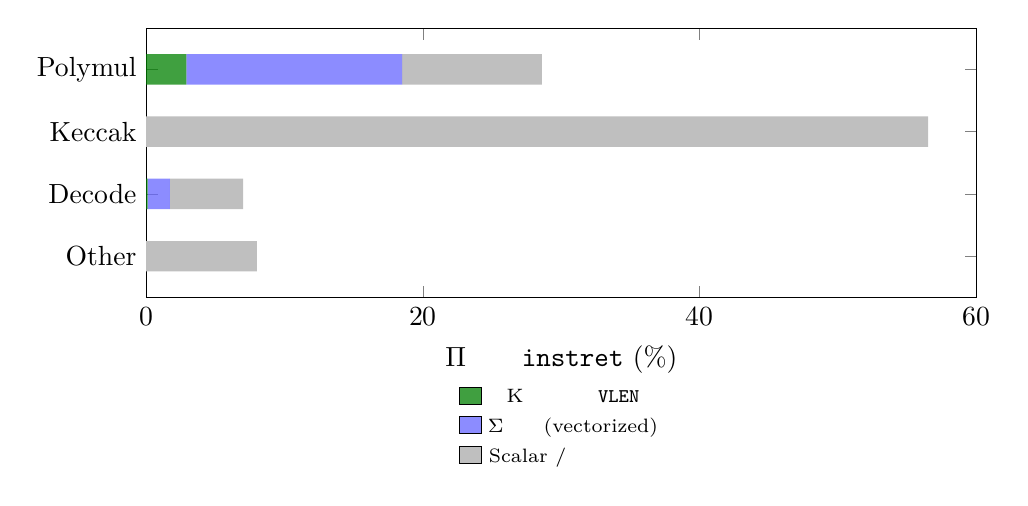
\begin{tikzpicture}
      \begin{axis}[
        width=\linewidth, height=5.0cm,
        xbar stacked, bar width=11pt,
        symbolic y coords={Other,Decode,Keccak,Polymul},
        ytick=data, xmin=0, xmax=60, xtick={0,20,40,60},
        xlabel={Ποσοστό \instret (\%)},
        legend style={at={(0.5,-0.30)}, anchor=north, legend columns=1,
                      font=\scriptsize, draw=none},
        every axis plot/.append style={draw=none},
        enlarge y limits=0.22,
      ]
      \addplot[fill=green!50!black,fill opacity=0.75] coordinates {(2.9,Polymul) (0,Keccak) (0.1,Decode) (0,Other)};
      \addlegendentry{Κλιμακώνει με \VLEN}
      \addplot[fill=blue!60,fill opacity=0.75] coordinates {(15.6,Polymul) (0,Keccak) (1.6,Decode) (0,Other)};
      \addlegendentry{Σταθερό (vectorized)}
      \addplot[fill=gray!50] coordinates {(10.1,Polymul) (56.5,Keccak) (5.3,Decode) (8.0,Other)};
      \addlegendentry{Scalar / μη κλιμακούμενο}
      \end{axis}
      \end{tikzpicture}
      % src: results/simulation/profiling/hotspots/vector_Zvk/hotspots_kem_L128_vector-zvk_latest.csv (commit bdd9cf4)
    \end{column}
  \end{columns}
  \pdfpcnote{HQC-128, Tier3, VLEN=256: scalable 3.0\% / fixed-vec 17.2\% / scalar 79.9\%. Horizontal layout -> kernel labels no overlap.}
\end{frame}


\end{document}
